\chapter{A Contrast-Based Model of Reverse Sobel Sequence (In-)Felicity}\labch{pragmatics-SS}
In the preceding chapter, we have isolated the criteria that render reverse Sobel sequences either felicitous or infelicitous. The pertinent data was gathered from the literature, an original experiment, and further introspection. The pertinent isolated empirical criteria are as follows: (i)~Contrastive stress in the second antecedent is required for felicity; (ii)~some form of stress obligatorily falls upon the auxiliary verb if no lexical item in the second conditional's antecedent is overtly different from the first conditional's antecedent; (iii)~despite assuming contrastive stress, a reverse Sobel sequence is always infelicitous, if the proposition $\phi$ precedes $\psi$ on some causal chain of events; (iv)~assuming felicity-enabling previous factors (including an acausal relationship between $\phi$ and $\psi$), a reverse Sobel sequence is always felicitous if the closest $\phi\land\psi$-worlds are counterfactual by nature; and (v)~assuming appropriate contrastive stress, the denigration of $\phi\land\psi$'s possibility renders any reverse Sobel sequence felicitous, regardless of all other previously mentioned factors (barring contrastive stress itself).%

To capture these intuitions, we propose to make use of the following ingredients and tools from the literature: (i)~The antecedent of a conditional sets the current aboutness topic \parencite{Ebert2008}, not only for indicative and future-less-vivid conditionals but also for counterfactual ones \parencite[cf.][p.~139]{Ebert2008}; (ii)~\textit{would} is sensitive to modal subordination \parencite{Klecha2011,Klecha2014,Klecha2015}; (iii)~the focus value for pro-forms may be a set of identity functions over alternative domains \parencite{Jacobson2004}; (iv)~differences to the actual world that causally stem from another initial change do not further decrease the similarity of the world in question \parencite{Bennett2003,Arregui2009}; (v)~imprecision and precisification may affect the evaluation of a conditional with respect to its set of antecedent worlds \parencite{Klecha2014,Klecha2015}; and (vi)~any domain of universal quantification is contextually restricted to exclude contextually irrelevant worlds \parencites{Fintel1994}{Reimer1998}{Stanley2000}{Klecha2014}[amongst many others]{Klecha2015}.

\section{The Effect of Contrastive Stress in a Variably-Strict Semantics}\labsec{contrast-vss}
The observation that some form of stress is required appears crucial: It is the only known factor that inevitably leads to infelicity should its requirement not be fulfilled. As such, the mechanisms surrounding contrastive stress must be at the centre of any explanation of reverse Sobel sequence (in-)felicity, including the one we present in this section.

As shown in \refsec{ASS}, there are two different strategies to derive a valid form of stress in the second conditional's antecedent of a reverse Sobel sequence: We either need to contrastively stress some lexical item that is overtly different from a counterpart in the preceding antecedent, or we have to stress the auxiliary verb of the reverse Sobel sequence's $\phi$-conditional. First, let us revisit the former case. Consider \refex{contrast-host}, repeated below as \refex{contrast-host-2}:
\pex\labex{contrast-host-2}\vspace{-9.5mm}
\a\speaker{Ben}If Karlos had hosted the party, it would not have been a good time.
\a\speaker{Martina}But if Karlos had \MakeUppercase{come} to the party, it would have been a good time.\hfill\parencite[p.~151]{Klecha2014}
\xe
As previously mentioned in \refsec{ASS}---as it was originally argued by \textcite[p.~52]{Klecha2014}---the contrastive stress on \textit{come} may lead to an exhaustified reading such as the one in \refex{contrast-host-exh}.
\pex
\a\speaker{Ben}If Karlos had hosted the party, it would not have been a
good time.
\a\speaker{Martina}But if Karlos had \MakeUppercase{come} to \textit{(but not hosted)} the party, it would have been a good time.\labex{contrast-host-exh}
\xe
Therefore, it is apparent why such reverse Sobel sequences might be felicitous: The set of the closest $\phi\land\psi$-worlds and the set of the closest $\phi\land\neg\psi$-worlds are, by definition, disjoint. This would prevent any inconsistent readings from arising from the semantics of the reverse Sobel sequence.

Now, let us revisit the second case: We have shown in \refsec{ASS} that some form of stress may occur even for reverse Sobel sequences where the second conditional's antecedent does not contain any lexical item that overtly differs from the first conditional's antecedent. In such cases, stress appears to obligatorily shift to the auxiliary verb, if present. The question would be why it is the auxiliary verb that is stressed. There appear to be three salient possibilities: 

First, an auxiliary verb is often contrastively stressed to contrast its clause's positive polarity against a preceding clause's negative polarity (see \citeauthor{Romero2004}, \citeyear{Romero2004}, p. 629; \citeauthor{Grimshaw2013}, \citeyear{Grimshaw2013}; \citeauthor{Wilder2013}, \citeyear{Wilder2013}; amongst others), as shown in \refex{positivepolarityfocus}
\ex
Everybody who didn't finish on time met with \MakeUppercase{John}, but everybody who \MakeUppercase{did} finish on {ti}me met with {Ma}ry.\\\emptyfill\parencite[adapted from][p.~630]{Romero2004}\labex{positivepolarityfocus}
\xe
It should be noted that---whilst the auxiliary verb is stressed to contrast positive polarity against negative polarity---the contrastive stress naturally falls upon the negation of its clause, if its negative polarity is to be contrasted against some preceding clause's positive polarity, as demonstrated by \refex{negativepolarityfocus}.
\ex
Everybody who finished on \MakeUppercase{ti}me met with \MakeUppercase{Ma}ry, and everybody who did \MakeUppercase{not} finish on time met with \MakeUppercase{John}.\hfill\parencite[p.~630]{Romero2004}\labex{negativepolarityfocus}
\xe
So, how does this fit into the antecedental stress exhibited by reverse Sobel sequences? It would seem that it does not. For starters, a reverse Sobel sequence does not exhibit a change in antecedent polarity between its $\phi\land\psi$-conditional and its subsequent $\phi$-conditional. The only difference is a difference in which worlds are explored and which consequences are predicted---there is no reason to assume that the $\phi$-conditional is contrasted against even an implicit $\neg\phi$-conditional. As such, we would rule out polarity focus as a potential option for reverse Sobel sequences.

Second, closely related to polarity focus, a stressed auxiliary verb may also signify verum focus \parencite{Hohle1992,Richter1993,Romero2004}. Contrary to the previous type of polarity focus, here, we do not contrast the positive polarity against a preceding clause's negative polarity, but rather emphasise that the speaker is certain that the proposition expressed by the clause should be added to the common ground \parencite{Hohle1992,Gutzmann2011,Romero2004,Romero2015,Gutzmann2020}. This intuition is shown in \refex{verumexample}, where the accented auxiliary verb appears to clarify the epistemic certainty of \textit{Kimiko went to the Himalayas}, after it was indirectly called into question by some previous speaker. In this sense, it is more akin to a contrast in epistemic certainty, rather than a contrast in polarity, compared to our examples \refex{positivepolarityfocus} and \refex{negativepolarityfocus}.
\pex\labex{verumexample}\vspace{-9.5mm}
\a \speaker{A} Peter claims Kimiko went to the Himalayas.\\
\speaker{S} She \MakeUppercase{did} go to the Himalayas.\\\emptyfill\parencite[adapted from][p.~630]{Romero2004}
\a \speaker{A} Peter doesn't think Kimiko went to the Himalayas.\\
\speaker{S} She \MakeUppercase{did} go to the Himalayas.\\\emptyfill\parencite[adapted from][p.~630]{Romero2004}
\xe
It is easy to see how a verum-based analysis might be attractive in terms of correctly deriving the (in-)felicity of certain reverse Sobel sequences: Let us assume that verum focus introduces a covert operator {\scshape verum}, as defined by \textcite{Romero2004}:
\ex
$\intension[gx/i]{{\scshape verum}\textsubscript{i}} = \lambda{p_{s,t}}.\lambda{w_s}.\forall{w'\in\text{Epi}_x(w)}[\forall{w''\in\text{Conv}_x(w')}[p\in CG_{w''}]]$
\xe
Here, $\text{Epi}_x(w)$ would be the set of worlds conforming to $x$’s knowledge in $w$; $\text{Conv}_x(w')$ is the set of worlds where all of $x$'s conversational goals in $w'$ are fulfilled (e.g., attaining maximal information whilst preserving truth); and where $\text{CG}_w''$ is the common ground; i.e.,~the set of propositions that the speakers assume in $w''$ to be true \parencite{Stalnaker1978}.

However, a {\scshape verum}-based analysis would present a number of issues: To know whether or not the stress on the auxiliary verb is actually a case of verum focus, we must look at the known effects of {\scshape verum} in the antecedents of conditionals. For example, \textcite[p.~533]{Romero2015} observed that {\scshape verum} appears to render conditionals that make use of counterfactual morphology to lead to a non-counterfactual conclusion (hereafter referred to as Anderson-style conditionals) infelicitous. This was demonstrated via two phenomena that, in conditionals, are nearly unambiguously known to be instances of {\scshape verum}: the particle \textit{really}---which is identical in meaning to {\scshape verum} \parencite[p.~625]{Romero2004}---and high negation in the antecedent. First, we demonstrate \citepos{Romero2015} observed effect of {\scshape verum} on Anderson-style conditionals with \textit{really} with the contrasting conditionals in \refex{anderson} and \refex{anderson-verum-really}:
\pex
\a If Jones had taken arsenic, he would have shown the symptoms that he indeed showed. So, it is likely that he took arsenic.\hfill\parencite{Anderson1951}\labex{anderson}
\a\ljudge{\#} If Jones really \MakeUppercase{had} taken arsenic, he would have shown the symptoms that he indeed showed. So, it is likely that he took arsenic.\labex{anderson-verum-really}
\xe
Second, we demonstrate \citepos{Romero2015} observed effect of {\scshape verum} on Anderson-style conditionals with high negation in the antecedent with the contrast between \refex{nevergonnausethisagain1} and \refex{nevergonnausethisagain2}:
\pex
\a If there hadn’t\textsubscript{Low} been any / had been no\textsubscript{Low} oil in the tank, the furnace would have made exactly the noise that it in fact did. So, it’s likely that the tank was empty.\hfill\parencite[p.~521]{Romero2015}\labex{nevergonnausethisagain1}
\a \ljudge{\#} If there hadn’t\textsubscript{High} been some\textsubscript{PPI} oil in the tank, the furnace would have made exactly the noise that it in fact did. So, it’s likely that the tank was empty.\hfill\parencite[p.~521]{Romero2015}\labex{nevergonnausethisagain2}
\xe
As such, if the stressed auxiliary verb in reverse Sobel sequences were to actually induce verum focus, it should follow that an Anderson-type reverse Sobel sequence should be infelicitous. However, if we consider the acausal counterfactual Anderson-type reverse Sobel sequence in \refex{anderson-rss}, this prediction does not bear out.
\ex\context{In a situation where the speaker tries to determine what caused Jones symptoms, where they disagree with another speaker's argument that arsenic could not be responsible if Jones was immune to its effects.}
Yes, if Jones had taken arsenic and he had been immune to its effects, he would not have shown the symptoms that he indeed showed; but if Jones \MakeUppercase{had} taken arsenic, he \MakeUppercase{would} have shown the symptoms that he indeed showed. So, it \MakeUppercase{is} likely that he \MakeUppercase{did} take arsenic.\labex{anderson-rss}
\xe
Therefore, we tentatively exclude verum focus as a possible candidate, as reverse Sobel sequences fail to pattern with other known cases of {\scshape verum}.%

The third focus option would be a contrastive tense-aspect-mood (hereafter TAM) focus, as is possible with stress on auxiliary verbs \parencite[p.~12f, footnote~3]{Goodhue2018}. Such contrastive focus is most frequently used to contrast a difference in tense: E.g., by emphasising that some proposition does not apply to the present, but to the past, as demonstrated by \refex{tensefocus}:
\pex
\speaker{A} Dinah is buying yogurt.\labex{tensefocus}
\a \speaker{B} No, she \MakeUppercase{was} buying yogurt.
\a \speaker{B} No, she (already) \MakeUppercase{did} buy yogurt.\\\emptyfill\parencite[p.~13, footnote~3]{Goodhue2018}
\xe
But how would this apply to reverse Sobel sequences? If we recall, the majority of reverse Sobel sequences use the same tense, aspect, and mood for both conditionals. Furthermore, most reverse Sobel sequences also refer to the same time interval, rather than, for example, two different points in the past. Instead, they rather refer to different possibilities for the same time interval---in the case of acausal counterfactual reverse Sobel sequences,  they refer to differently remote possibilities for the same time interval. Here, it is important to recall that TAM morphology in conditionals is connected to the properties of the world variable \parencites{Palmer1986}{Iatridou2000}{Arregui2009}{Romero2014}[amongst others]{Schulz2014}. We propose that the stress on the auxiliary verbs in reverse Sobel sequences targets exactly that part in meaning: the properties of the world variable $w$ which impact the quantificational domain of the conditional. If this is indeed the case, then \citepos{Klecha2014} general observation regarding the necessity of contrastive stress can be extended to these cases as well, and the underlying form of stress for all felicitous reverse Sobel sequences would be a form of contrastive stress/focus. However, before we further explore this concept in \refsec{proform}, we first take a look at modal subordination and aboutness topicality in \refsec{modal}.

\subsection{Modal Subordination}\labsec{modal}
First, we must answer the question of why reverse Sobel sequences tend to be infelicitous without contrastive stress, even if the two conditionals should, in theory, quantify over two differing levels of world closeness. Here, we would argue that \textcite{Klecha2014,Klecha2015} is correct with his suggestion that modal subordination might be the culprit.\footnote{Note that \textcite{Klecha2014,Klecha2015} only explicitly suggested modal subordination to apply to acausal reverse Sobel sequences. However, there is no reason not to apply it to all kinds of reverse Sobel sequences: After all, if \textit{would} is sensitive to modal subordination, it should occur regardless of causality.} That \textit{would} is actually sensitive to modal subordination is demonstrated by \refex{modalsubordination}, where the \textit{would} of the second sentence is interpreted with respect to the context established by the preceding sentence.
\ex 
My family used to go to Albion. We would drive through Ontario.\\\emptyfill\parencite[p.~378]{Klecha2011} \labex{modalsubordination}
\xe
\textcite{Klecha2014,Klecha2015} argues that this would affect the interpretation of a reverse Sobel sequence as follows: \enquote{If $\phi\land\psi$, $\neg\chi$; but if $\phi$, $\chi$} is interpreted as \enquote{If $\phi\land\psi$, $\neg\chi$; but if $\phi\land(\phi\land\psi)$, $\chi$}, which would render the $\phi$-conditional contradictory to the preceding $\phi\land\psi$-conditional. Essentially, this would mean that the $\phi$-conditional of a reverse Sobel sequence is interpreted with respect to the $\phi\land\psi$-conditional's domain of quantification, rather than establishing its own. 

First, we must ponder the question of when any conditional should be analysed with respect to a preceding conditional's antecedent: If we compare the subordinated example \refex{sobelesque} to the non-subordinated example \refex{nonsense-subordination}, there are two clear differences between them. 

\ex
\context{John is married to Mary. He is a good liar and a flirt. Because of this, Mary always suspected him of cheating and once contemplated hiring a very competent private investigator but ultimately decided against it. However, John has never actually cheated on Mary, unbeknownst to her. Sue knows all of this.}
\speaker{Sue}If John had cheated on Mary, she would've never found out about it; but if she had hired the private investigator, he would've brought her evidence of John's cheating.\labex{sobelesque}
\xe
\ex
\speaker{Sue}If John had killed his boss, he would've spent his summer in prison; but if John had won the lottery, he would've gone on a cruise around the world.\labex{nonsense-subordination}
\xe

The first difference is as follows: For \refex{sobelesque}, both conditionals appear to be topically related, as both can be interpreted as exploring the question of what would have happened had John cheated on his wife, going through different scenarios. For \refex{nonsense-subordination}, most people would have trouble coming up with a topical relation between the two conditionals: One explores what would have happened to John had he murdered his boss, whereas the other one explores what would have happened had he won the lottery.

The second difference is as follows: For \refex{sobelesque}, the consequent of the second conditional requires a modally subordinate reading. Without it, the conditional would be evaluated as false. For \refex{nonsense-subordination}, this is not the case. Traditional analyses would suggest, however, that modal subordination is not contingent upon the resulting reading's felicity \parencite{Roberts1987,Roberts1989}. Indeed, if we alter \refex{sobelesque} such that the second conditional's consequent is contradictory to the first conditional's antecedent, the modally subordinate reading appears to remain intact, yielding an infelicitous sequence, as seen below in \refex{sobelesque-bad}.
\ex
\context{John is married to Mary. He is a good liar and a flirt. Because of this, Mary always suspected him of cheating and once contemplated hiring a very competent private investigator but ultimately decided against it. However, John has never actually cheated on Mary, unbeknownst to her. Sue knows all of this.}
\speaker{Sue}If John had cheated on Mary, she would've never found out about it;\linebreak\ljudge{??} but if she had hired the private investigator, he would've told her that John didn't cheat on her.\labex{sobelesque-bad}
\xe
As such, modal subordination does not take into account whether or not its presence is advantageous or disadvantageous. Rather, modal subordination is solely determined by whether or not a conditional can be interpreted as topically related to the antecedent of its preceding conditional.

This observation fits well with \citepos{Ebert2008} claim that the antecedent of a conditional serves as an topic-introducing device. \textcite{Ebert2008,Ebert2014} argued that the antecedent of a fronted conditional sets the aboutness topic of the current discourse; i.e.,~it sets the topic by which the consequent is evaluated. We would argue that the first conditional's antecedent sets the aboutness topic as described by \textcite{Ebert2008,Ebert2014}, but that any subsequent conditional is interpreted as merely elaborating upon the previously established topic, if at all possible, thereby establishing a subordinating discourse relation between the two conditionals in question \parencite{Asher2005}.\footnote{An alternative approach in explaining this behaviour might lie with \textcite{Eckardt2021}, who proposes a DRT account which incorporates a world discourse referent that may be maintained over multiple sentences. We propose further research in that direction.}

This would explain (i)~why \refex{sobelesque} and \refex{sobelesque-bad} are modally subordinated, (ii)~why \refex{nonsense-subordination} is not, and (iii)~why reverse Sobel sequences are subjected to modal subordination by default: It is difficult to conceive that the $\phi$-antecedent's proposed topic could ever be considered incompatible to the pre-established aboutness topic of the $\phi\land\psi$-antecedent.

To establish a non-subordinating discourse relation in such cases, it would then appear necessary that the speaker provides some overt cue that clarifies that the new conditional should be interpreted with regards to its own particular aboutness topic, rather than the previously established one. We argue that this is accomplished via the contrastive stress that appears mandatory to felicitous reverse Sobel sequences. The reasoning concerning this is rather simple: Contrastive stress with regards to topic is referred to as contrastive topic in the literature \parencite{Buring1997,Buring2003,Krifka2007,Buring2016,Constant2012}, and contrastive topic, by definition, introduces a new topic that is clearly demarcated from any previous topic (that is, contrastive topic clarifies that its topic answers part of topical space that was hereto left unaddressed), cancelling the latter's actuality \parencite{Ebert2008,Krifka2007,Ebert2014,Lee2017,vanRooij2017,Yabushita2017} and thereby forces a non-subordinate discourse relation between itself and the previous sentence. \textcite[p.~44ff]{Krifka2007}, specifically, covers the use of contrastive topic for aboutness topics. An example of this is shown in \refex{krifka-cs}.
\pex\label{ex:krifka-cs}
\a \speaker{A}What do your siblings do?
\a \speaker{B}[My [\MakeUppercase{si}ster]\textsubscript{Focus}]\textsubscript{Topic} [studies \MakeUppercase{med}icine]\textsubscript{Focus},
and\\\phantom{\speaker{B}}[my [\MakeUppercase{bro}ther]\textsubscript{Focus}]\textsubscript{Topic} is [working on a \MakeUppercase{freight} ship]\textsubscript{Focus}.\\\emptyfill\parencite[adapted from][p.~44]{Krifka2007}
\xe
In order for the contrastive topic to be successful, however, we require that the two contrasted items do not topically overlap. E.g., for \refex{krifka-cs}, we would require that the topic of his sister and the topic of his brother are non-overlapping. If this is violated, as in \refex{krifka-cs-bad}, where the later topic is a subset of the earlier topic, its use is infelicitous.
\pex\label{ex:krifka-cs-bad}
\a \speaker{A}What do your siblings do?
\a \speaker{B}\phantom{\#}[My [\MakeUppercase{bro}thers]\textsubscript{Focus}]\textsubscript{Topic} [study \MakeUppercase{med}icine]\textsubscript{Focus},
and\\\phantom{\speaker{B}}\#[my [\MakeUppercase{lit}tle brother]\textsubscript{Focus}]\textsubscript{Topic} is [working on a \MakeUppercase{freight} ship]\textsubscript{Focus}.\\\emptyfill\parencite[p.~267]{Krifka2007}
\xe

In \refch{pragmatics-SS}, we have established that contrastive stress obligatorily falls upon the antecedent's auxiliary verb, should no other overtly different lexical item be available. Given reasoning concerning modal subordination above, we would assume that a contrastively stressed auxiliary verb must suffice to prevent a modally subordinate reading in order for such reverse Sobel sequences to be felicitous. Indeed, additional data supports the view that contrastive stress on the auxiliary verb cancels modally subordinate readings in conditionals. Compare \refex{sobelesque} and \refex{sobelesque-bad}, repeated below as respectively \hyperref[ex:nananana-batman1]{(\ref*{ex:nananana-batman1}-i)} and \hyperref[ex:nananana-batman1]{(\ref*{ex:nananana-batman1}-ii)}, to their respective counterparts in \hyperref[ex:nananana-batman3]{(\ref*{ex:nananana-batman3}-i)} and \hyperref[ex:nananana-batman3]{(\ref*{ex:nananana-batman3}-ii)}, where contrastive stress was added to the auxiliary verb.
\pex
\contextpex{John is married to Mary. He is a good liar and a flirt. Because of this, Mary always suspected him of cheating and once contemplated hiring a very competent private investigator but ultimately decided against it. However, John has never actually cheated on Mary, unbeknownst to her. Sue knows all of this.}
\a \pextitle{Without Contrastive Stress:}\beginsubsub
\b{i.} \speaker{Sue}If John had cheated on Mary, she would've never found out about it; but if she had hired the private investigator, he would've brought her evidence of John's cheating.\labex{nananana-batman1}
\b{ii.} \speaker{Sue}If John had cheated on Mary, she would've never found out about it; {??}but if she had hired the private investigator, he would've told her that John didn't cheat on her.\labex{nananana-batman2}
\endsubsub\pagebreak
\a \pextitle{With Contrastive Stress:}\beginsubsub
\b{i.} \speaker{Sue}If John had cheated on Mary, she would've never found out about it; {??}but if she \MakeUppercase{had} hired the private investigator, he would've brought her evidence of John's cheating.\labex{nananana-batman3}
\b{ii.} \speaker{Sue}If John had cheated on Mary, she would've never found out about it; but if she \MakeUppercase{had} hired the private investigator, he would've told her that John didn't cheat on her.
\endsubsub
\xe
Here, the acceptability of each sequence appears to be inverted by the introduction of contrastive stress\footnote{Again, it should be noted that the feedback I received on this from native speakers ($n=3$) was mixed. Whilst most considered the infelicitous sequences in \hyperref[ex:nananana-batman1]{(\ref*{ex:nananana-batman1}-ii)} and \hyperref[ex:nananana-batman3]{(\ref*{ex:nananana-batman3}-i)} significantly degraded, a minority found the sequence in \refex{nananana-batman3} only slightly less acceptable than \refex{nananana-batman1}. The trend appears clear regardless.}---which would be in line with a non-subordinated reading: After all, the private investigator cannot bring evidence of John's cheating if we do not carry over the previous conditional's counterfactual assumption that John had, in fact, cheated on Mary in \hyperref[ex:nananana-batman3]{(\ref*{ex:nananana-batman3}-i)}. As such, it is clear that a validly contrastively stressed auxiliary verb should suffice to prevent modal subordination within reverse Sobel sequences. However, not all contrastively stressed reverse Sobel sequences are actually felicitous. We must therefore face the question of what the formal semantics of contrastive stress in reverse Sobel sequences is---and how contrastive stress still derives infelicity in certain cases. We explore the former question in \refsec{proform}, before tackling the specifics of the latter question in \refsec{showitworks}.

\subsection{Auxiliary Verbs and the Focus Value of Pro-Forms}\labsec{proform}
In order to establish the felicity conditions for contrastive stress on auxiliary verbs, we must first take a look at the role auxiliary verbs play in the semantics of conditionals. At least in the English language, it is a generally uncontroversial claim to say that top-level auxiliary verbs encode the TAM information of their respective clause \parencites{Chomsky1957}{Akmajian1979}[amongst others]{Klein1994}, if present. It is furthermore generally accepted that TAM morphology is crucially connected to the domain world selection process of conditionals \parencites{Palmer1986}{Iatridou2000}{Arregui2009}{Romero2014}{Schulz2014}; e.g., by marking a conditional as either indicative, future-less-vivid, or counterfactual by nature. See the following minimal pair of example conditionals in \refex{kennedy}, due \textcite[p.~90]{Adams1970}:
\pex\label{ex:kennedy}
\a If Oswald didn't shoot Kennedy, someone else did.\labex{kennedy-indicative}
\a If Oswald hadn't shot Kennedy, someone else would have.\labex{kennedy-subjunctive}
\xe
The indicative in \refex{kennedy-indicative} makes an epistemic claim: The speaker may not be certain whether or not it was Oswald that shot Kennedy, but someones most certainly did. A statement that would be considered true by anyone who knows that Kennedy was, in fact, shot. The counterfactual subjunctive in \refex{kennedy-subjunctive}, on the other hand, makes a metaphysical claim about how the world would have worked: The speaker takes it for granted that it was, in fact, Oswald who shot Kennedy, but makes the claim that, had he not, someone else would have done so. Contrary to the indicative, this sentence would only be considered true by someone who believes that our world was structured in such a way that Kennedy's assassination was inevitable (e.g., by believing in a grand conspiracy or some such). As such, the TAM morphology---the only overtly differing factor between \refex{kennedy-indicative} and \refex{kennedy-subjunctive}---appears to impact the conditionals' domain of quantification: TAM morphology marks whether we quantify over a set of epistemic worlds or over a set of metaphysical worlds \parencite[see, amongst others,][p.~62]{Condoravdi2002}.


Despite a substantial amount of literature on the topic, there appear to be varying degrees of consensus on the specifics of the TAM morphology's semantic contribution; from which part of TAM semantics is actually present in any given conditional to which part of TAM morphology carries which specific semantics and what these specific semantics actually even are \parencite{Fintel1997,Fintel2001,Dudman1983,Dudman1984,Iatridou2000,Arregui2007,Anand2010,Schulz2014}. Originally, the semantics of TAM morphology was treated as a single, undifferentiated chunk \parencite{Stalnaker1975,Fintel1997}. Later work attempted to differentiate between the contribution of tense, mood, and aspect. Currently, the semantic contributions of aspect \parencite{Hacquard2006,Arregui2007,Anand2010} and mood \parencite{Romero2017}---for languages with proper mood---are relatively well-understood. Concerning tense, however, there are, at the moment, two different main lines of thought: One main line of thought is that tense morphology marks one form or another of \enquote{modal remoteness}, as pertaining to the world variable \parencite{Stalnaker1975,Palmer1986,Iatridou2000,Huddleston2002,Schulz2014}. In these cases, counterfactual TAM morphology may indicate that the antecedent worlds are not necessarily live possibilities of the conversants \parencite{Stalnaker1975,Fintel1997} or that the actual world is excluded from evaluation regardless of antecedent-compliance \parencite{Iatridou2000,Schulz2014}. The other main line of thought considers tense morphology to mark the \enquote{temporal remoteness} of the antecedent worlds---evaluating the conditional either with respect to present possibilities for non-counterfactual conditionals or with respect to possibilities of some earlier time for counterfactual conditionals \parencite{Dudman1983,Dudman1984,Ippolito2003,Arregui2009,Gronn2009,Romero2014,Romero2017}. For the purposes of this dissertation, we remain agnostic about the exact nature and distribution of the meaning of TAM morphology, but retain the common denominating factor---namely, that TAM morphology restricts and selects the set of evaluation worlds from the set of all compatible antecedent worlds in one way or another.

In reverse Sobel sequences, the TAM morphology of the auxiliary verbs would yield different semantic values that could be contrasted against: One auxiliary verb's TAM morphology restricts the domain of quantification to the closest $\phi\land\psi$-worlds, whereas the other auxiliary verb's TAM morphology restricts the domain of quantification to the closest $\phi$-worlds. As these two sets should always be non-identical so long as $\phi\neq\psi$, one could argue that the contrast should always succeed and that any reverse Sobel sequence with contrastive stress on the auxiliary verb be rendered felicitous (barring other intervening factors). It would appear, however, that non-identicality is insufficient, considering the plenitude of infelicitous reverse Sobel sequences seen in \refsec{introspection} (e.g., non-denigrated counterfactual causal reverse Sobel sequences and non-denigrated non-counterfactual reverse Sobel sequences are infelicitous regardless of contrastive stress). It would appear that the two contrasting domains must not only be non-identical but rather entirely disjoint for a successful contrast (as the reverse Sobel sequence would yield a logical contradiction otherwise). As such, we require a semantic mechanism that ideally not only enforces non-identicality but also facilitates disjointness to escape modal subordination and to thereby also escape contradictory readings. In other words, we require the $\phi$-conditional to be interpreted as using a $\phi\land\neg\psi$-domain (without overtly placing the $\neg\psi$ in the antecedent) to be disjoint to the preceding $\phi\land\psi$-domain. We previously saw this facilitated in, e.g., \refex{match}, repeated below as \refex{match-s2-repeat}, where the second antecedent is interpreted as restricting our claim to worlds in which the speaker had struck the match and where we maintain the fact that the match was dry.
\ex\labex{match-s2-repeat}\context{Holding up a dry match, with no water around.}If I had struck this match and it had been soaked, it would not have lit. But if I had struck this match, it would have lit.\\%
\emptyfill(adapted from \textcite[p.~106]{Stalnaker1968} by \textcite[p.~487]{Lewis2018})
\xe

In this regard, reverse Sobel sequences behave strikingly similar to contrastively stressed bound pro-nouns, which also not only require non-identical contrasting domains, but contrasting domains that are, in fact, disjoint \parencite{Sauerland1998,Sauerland1999,Sauerland2000,Jacobson2000,Jacobson2004,Mayr2012}. Therefore, we would argue that a successful analysis of contrastively stressed TAM moprhology patterns along the lines of analyses regarding contrastively stressed bound pro-forms.

To this end, we make a brief excursion to the semantics of bound pronouns with contrastive stress: \textcite{Sauerland1998,Sauerland1999} argued for the existence of indices in the grammar using sentences such as \refex{sauerland}, where bound pronouns were focused via contrastive stress.
\ex
Every fourth grade boy$_i$ called his$_i$ mother, but no \MakeUppercase{fifth} grade boy$_j$ called \MakeUppercase{his}$_j$ mother.\labex{sauerland}
\xe
However, as noted by \textcite{Jacobson2000,Jacobson2004} and \textcite{Sauerland2000} himself, this does not appear to be a case of simply contrasting differing indices: Contrastively bound pronouns appear to be illicit when their binders may be different but still overlapping in their domain, as demonstrated by \refex{sauerland-domain}.
\ex
\ljudge{*}I expected every student\textsubscript{i} to call his\textsubscript{i} father, but only every \MakeUppercase{young} student\textsubscript{j} called \MakeUppercase{his}\textsubscript{j} father.\hfill\parencite[p.~206]{Sauerland1998}\labex{sauerland-domain}
\xe
\textcite{Jacobson2000,Jacobson2004} used this to argue for an alternate analysis of focused pronouns: She argues that contrastively stressed pronouns may give rise to two different sets of alternatives:  When not contrasted against another bound pronoun, the set of alternatives typically consists of the pronoun function from an individual to self (i.e.,~the identity function) and functions that map that individual to someone else, deriving a contrast this way. An example of such a case can be seen in \refex{jacobson-contrast-identity}.
\ex
Every fourth grade boy loves Jack's mother, and every fifth grade boy$_j$ loves \MakeUppercase{his}$_j$ mother.\labex{jacobson-contrast-identity}
\xe
When a pronoun is contrasted against another bound pronoun, the set of alternatives consists of (partial) identity functions of different domains, mapping elements of their restricted domain to themselves, deriving an obligatory contrast in domains between the two pronouns.
\pex
\a $\intension[g,c]{his\textsubscript{1}}$ is defined if $g(1)\in{D_R}$, where $D_R$ is the domain that binds the pronoun. When defined, $\intension[g,c]{his\textsubscript{1}}=g(1)$.
\a $\intension[g,c]{his\textsubscript{1}}=\predicate{id\textsubscript{R}}(g(1))$
\a $\intension[f,g,c]{his\textsubscript{1}}=\{\predicate{id\textsubscript{R'}}(g(1))~|~\predicate{id\textsubscript{R'}}\subseteq \predicate{id}_{\langle e,e\rangle}\}$
\xe
Crucially, \textcite{Jacobson2000,Jacobson2004} posits that the two contrasting (partial) identity functions' domains of definition must be non-overlapping (i.e.,~there is no element that is mapped by both identity functions to either itself or any other defined value). An unsuccessful example of this type of contrast was already shown in \refex{sauerland-domain}, where one domain was the subset of the other, and a successful example of this type of contrast was shown in \refex{sauerland}. The corresponding LFs are shown in \refex{jacobsonex2}, where the contrasting elements are highlighted in boldface.
\pex\label{ex:jacobsonex2}
\a every 3\textsuperscript{rd}-grader $[\lambda x.\predicate{call}(x, \predicate{the-mother-of}(\predicate{\textbf{\color{black}id\textsubscript{3rd-graders}}}(x)))]$
\a every 4\textsuperscript{th}-grader $[\lambda x.\predicate{call}(x, \predicate{the-mother-of}(\predicate{\textbf{\color{black}id\textsubscript{4th-graders}}}(x)))]$
\xe

\textcite{Jacobson2000,Jacobson2004} further argues for the existence of these two readings using sentences where contrastive stress is placed upon a reflexive pronoun, where the two different readings manifest themselves as variant stress patterns: If the contrast between the mapping from an individual to self vs. others is desired, the contrastive stress falls upon the \textit{self} of the reflexive pronoun, as shown in \refex{identity-good}. If, on the other hand, the contrast between domains is required, then the contrastive stress falls upon the pro-form part of the reflexive pronoun, as shown in \refex{domain-good}.
\pex
\a Every third grade boy loves Mary, and every \MakeUppercase{fourth} grade boy loves him\MakeUppercase{self} (as opposed to someone else). \labex{identity-good}
\a Every third grade boy loves himself, and every \MakeUppercase{fourth} grade boy loves \MakeUppercase{him}self \labex{domain-good}
\emptyfill\parencite[adapted from][p.~68]{Jacobson2000}
\xe
This placement of contrastive stress appears obligatory, as using the opposite stress pattern for either case would yield illicit readings, as shown in \refex{identity-bad} and \refex{domain-bad}.
\pex
\a\ljudge* Every third grade boy loves Mary, and every \MakeUppercase{fourth} grade boy loves \MakeUppercase{him}self.\labex{domain-bad}
\a\ljudge* Every third grade boy loves himself, and every \MakeUppercase{fourth} grade boy loves him\MakeUppercase{self} (*as opposed to someone else).\labex{identity-bad}\\
\emptyfill\parencite[adapted from][p.~68]{Jacobson2000}
\xe
Of these two readings, only the contrast in domains is of any relevance to the topic of reverse Sobel sequences---we would, therefore, refer to \textcite{Jacobson2000} for information on the other type of contrast.

How does this relate to the contrastive stress placed upon the auxiliary verb for reverse Sobel sequences? As previously stated, we would argue that contrastive stress or focus on an antecedent's auxiliary verb's TAM morphology evokes a value akin to bound pronouns that are contrastively stressed against another bound pronoun. Tense, for example, is often treated as a type of pro-form, as shown in \refex{tense}---e.g., by \textcite{Partee1973} and \textcite{Kratzer1998} amongst many others.
\ex 
$\intension[g,c]{\scshape past\textsubscript{i}}$ is defined only if $g(i)$ temporally precedes $t_0$, where $g(i)$ refers to the event time and $t_0$ refers to the actual time.\footnote{This definition corresponds to an absolute tense reading for the sake of simplicity. For a relative treatment of tense, see \textcite{Kusumoto1999}.}\\If defined, $\intension[g,c]{\scshape past\textsubscript{i}}=g(i)$\hfill\parencite[adapted from][p.~378]{Romero2017}.\labex{tense}
\xe
In addition, mood has also been treated as a type of pro-form in the literature, as shown in \refex{mood}---e.g., by \textcite{Schlenker2004,Schlenker2005}, who treated mood as pro-worlds.
\ex
$\intension[g,c]{\scshape indicative\textsubscript{i}}$ is defined only if $g(i)\in\predicate{dox\textsubscript{speaker}}$, where $\predicate{dox\textsubscript{speaker}}$ is the speaker's doxastic set of possible worlds.\\If defined, $\intension[g,c]{\scshape indicative\textsubscript{i}}=g(i)$\hfill\parencite[adapted from][p.~379]{Romero2017}.\labex{mood}
\xe
Now, in relation to reverse Sobel sequences, we would argue that focus on TAM-inflected verbs does not yield a set of alternative TAM-inflected verbs but rather a set of alternative domains---i.e.,~focus actually targets the domains of bound pronouns and the inflected TAM morphology rather than the focused items' stem meanings themselves. %
Let us recall that TAM morphology appears to be (at least partially) responsible for the world selection function of conditionals. As such, a contrastively stressed TAM verb should generate a set of salient alternative domain assignments that could, conceivably, have been used in place of the original conditional's domain of quantification. We show this is \refdef{tam}.
\pex\label{def:tam}
\a $\intension[g,c]{TAM\textsubscript{i}}$ is defined if $g(i)\in{D_R}$, where $D_R$ is the domain that binds the pro-form. When defined, $\intension[g,c]{TAM\textsubscript{i}}=g(i)$.
\a $\intension[g,c]{TAM\textsubscript{i}}=\predicate{id\textsubscript{R}}(g(i))$
\a $\intension[f,g,c]{TAM\textsubscript{i}}=\{\predicate{id\textsubscript{R'}}(g(i))~|~\predicate{id\textsubscript{R'}}\subseteq \predicate{id}_{\langle s,s\rangle}\}$
\xe
This set of alternatives would include the domain that it is contrasted against, as well as containing a number of less maximally similar antecedent compatible worlds. We also posit a presupposition to the contrastive stress that the two contrasting domains must be disjoint, inheriting this presupposition from the analysis of contrastively stressed bound pro-forms.\footnote{Note that whilst \textcite{Jacobson2000,Jacobson2004} herself does not provide an independent analysis for as to why disjoint domains should be required, there have been formal models that attempt to do so. We would refer to \textcite[p.~321 ff.]{Mayr2012} for one such account. We content ourselves with a simple presupposition of disjointness here, since the exact implementation that derives the requirement of disjoint domains is of no further consequence to the overall analysis.}

Having established what the alternatives to the auxiliary verb might be and what is required for a felicitous contrast, we may turn our attention to how the contrastive stress affects a reverse Sobel sequence: For the sequence \enquote{If $\phi\land\psi$, $\neg\chi$; but if {\scshape aux}\textsubscript{\scshape ct}-$\phi$, $\chi$}, the contrastive stress would attempt to contrast the set of the closest $\phi$-worlds against the salient counterpart of the preceding conditional: the set of the closest $\phi\land\psi$-worlds. As previously mentioned, due to the nature of the contrast, we would require the two contrasting domains to be disjoint. This is only the case if the $\phi$-conditional does not quantify over any of the closest $\phi\land\psi$-worlds, which, in turn, may only be the case---given a standard variably-strict analysis---if the two domains represent subsets of differing levels of world closeness. The respective LFs for a standard reverse Sobel sequence would therefore correspond to the LFs display in \refex{identityw}, where the contrasting identity functions are highlighted in boldface:
\pex\label{ex:identityw}
\a If $[\lambda w_s. \phi(\text{\textbf{\color{black}\scshape id\textsubscript{domain-b}}}(w))\land \psi(\text{\color{black}\scshape id\textsubscript{domain-b}}(w))]$, (then) $[\lambda w_s.\neg\chi(w)]$.
\a If $[\lambda w_s. \phi(\text{\textbf{\color{black}\scshape id\textsubscript{domain-a}}}(w))]$, (then) $[\lambda w_s.\chi(w)]$.
\xe
Where, as previously stated, in a variably-strict semantics domain A and domain B would correspond to the set of the closest $\phi$-worlds and the set of the closest $\phi\land\psi$-worlds, respectively, as shown in \refex{identityw-variably-strict}.
\pex\label{ex:identityw-variably-strict}
\a If $[\lambda w_s. \phi(\text{\textbf{\color{black}\scshape id\textsubscript{closest-$\phi\land\psi$}}}(w))\land \psi(\text{\color{black}\scshape id\textsubscript{closest-$\phi\land\psi$}}(w))]$, (then) $[\lambda w_s.\neg\chi(w)]$.
\a If $[\lambda w_s. \phi(\text{\textbf{\color{black}\scshape id\textsubscript{closest-$\phi$}}}(w))]$, (then) $[\lambda w_s.\chi(w)]$.
\xe
The formal implementation of which is shown in \refex{identityw-variably-strict-demo}, where the accessibility function $f_\leqslant(p,w)$ returns the set of $p$-worlds closest to the evaluation world $w$.
\pex\label{ex:identityw-variably-strict-demo}
\a $\intension{If $\phi$ and $\psi$, not $\chi$}=[\lambda w_s.\forall v:v\in f_\leqslant([\lambda w'_s.\phi(\text{\textbf{\color{black}\scshape id\textsubscript{closest-$\phi\land\psi$}}}(w'))$\\\emptyfill$\land\psi(\text{\textbf{\color{black}\scshape id\textsubscript{closest-$\phi\land\psi$}}}(w'))],w)[\neg\chi(v)]]$
\a $\intension{If $\phi$, $\chi$}=[\lambda w_s.\forall v:v\in f_\leqslant([\lambda w'_s.\phi(\text{\textbf{\color{black}\scshape id\textsubscript{closest-$\phi$}}}(w'))],w)[\chi(v)]]$
\xe

With this, we have established the felicity conditions for reverse Sobel sequences where the TAM-inflected verb is contrastively stressed---and thereby determined the factor that dictates whether or not modal subordination can be escaped: disjoint quantificational domains. The specifics on which reverse Sobel sequences fulfil these conditions are treated in the next section---i.e.,~\refsec{showitworks}.




But first, to summarise our position: We posit (i)~that the antecedent of a conditional sets the aboutness topic of the current discourse \parencite{Ebert2008,Ebert2014}; (ii)~that, in a sequence of conditionals, non-initial conditionals do not replace the established aboutness topic if there is some sensible way for their antecedent to correlate to it---causing non-initial conditionals to be analysed as modally subordinate to said aboutness topic; (iii)~that, if this is the case, contrastive stress is required as a cue to terminate the current aboutness topic and establish a new one---thereby cancelling modally subordinate readings (as motivated in \refsec{modal}); and (iv)~that contrastive TAM stress in the antecedent of conditionals is only felicitous if the contrasting conditionals' domains of quantification are disjoint to one another (as motivated in this section). In addition to what we have established in these sections, we also posit (v)~\citepos{Klecha2014,Klecha2015} model on causal Sobel sequences, including a world similarity metric \`a la \textcite{Bennett2003} and \textcite{Arregui2009}, as described in \refsec{CSS}; and (vi)~that domains of quantification are contextually restricted to exclude all worlds that are considered irrelevant to the discourse purpose \parencites{Fintel1994}{Reimer1998}{Stanley2000}{Klecha2014}[amongst many others]{Klecha2015}. We show in \refsec{showitworks} that these assumptions suffice to account for all known data presented in \refsec{introspection}, allowing for a uniform analysis of all felicitous reverse Sobel sequences assuming a single type of stress/focus in the antecedent of the second conditional.

\subsection{Retrodiction: Accounting for All Available Data With a Variably-Strict Semantics}\labsec{showitworks}
In order to test whether or not the model posited in \refsec{modal} and \refsec{proform} makes accurate predictions concerning the (in-)felicity of reverse Sobel sequences and regularly ordered Sobel sequences, we must first recall two important patterns of (in-)felicity: First, that all regularly ordered Sobel sequences are felicitous. Second, that the felicity of reverse Sobel sequences is dependent upon contrastive stress and three subordinate factors: causality, counterfactuality, and denigration. We established and summarised this in \refsec{introspection} in \reftab{ourdata}, repeated below as \reftab{ourdata-repeat}.

\begin{table}[!htb]
\input{content/tables/mydata}\labtab{ourdata-repeat}
\end{table}

\noindent Due to the greater theoretical importance of reverse Sobel sequence compared to regularly ordered Sobel sequences, we first tackle the (in-)felicity conditions of the former and then proceed to tackle the general felicity of the latter.

\subsubsection{Reverse Sobel Sequences}\labsec{vs-retro-rss}
In \refsec{modal}, we have argued that modal subordination is the default for all reverse Sobel sequences, leading to a contradictory reading due to both conditional antecedents quantifying over the same domain of worlds, and that reverse Sobel sequences require a successful contrastive stress in the antecedent to escape the subordinate reading, and thereby escape the contradictory reading cause by modal subordination. As argued for in \refsec{proform}, in order for the contrastive stress to be successful, we must be able to construct a domain that is disjoint from the preceding conditional's domain of quantification. Or, in set theoretical terms, contrastive stress on the auxiliary verb of a reverse Sobel sequence is felicitous iff $D_1\cap D_2=\emptyset$, where $D_1\subseteq D_{\text{closest-}\phi}$ and $D_2\subseteq D_{\text{closest-}\phi\land\psi}$. Here, $D_{\text{closest-}\phi}$ refers to the domain of worlds consisting of all maximally close $\phi$-worlds and $D_{\text{closest-}\phi\land\psi}$ refers to the domain of worlds consisting of all maximally close $\phi\land\psi$-worlds.

First, let us examine the effect of counterfactuality of $\phi\land\psi$ (note that we loop back to the effect of non-counterfactuality only later on). The example reverse Sobel sequences contrasting non-counterfactual ones with counterfactual ones, \refex{matchtomorrow} and \refex{match-repeat4}, are repeated below as \refex{doomsday-x} and \refex{doomsday-y}, respectively.
\ex\context{Concerning a dry match in a room with a large open source of water.}
    If I struck this match tomorrow and it was wet, it wouldn't light; \#but if I \MakeUppercase{were} to strike this match tomorrow, it would light.\labex{doomsday-x}
\xe
\ex\context{Holding up a dry match, with no water around.}If I had struck this match and it had been soaked, it would not have lit. But if I \MakeUppercase{had} struck this match, it would have lit.\\%
\emptyfill(adapted from \textcite[p.~106]{Stalnaker1968} by \textcite[p.~487]{Lewis2018})\labex{doomsday-y}
\xe
Our prime directive is to ensure the disjointness of the two domains of quantification. In the case of counterfactuality, it can be easily guaranteed that two domains of quantification are disjoint. For this to be the case, $\phi\land\psi$ and $\phi$ merely must possess differing degrees of similarity to the evaluation world to ensure that the closest $\phi$-worlds are $\phi\land\neg\psi$-worlds, since the world closeness ordering of counterfactual worlds is a mostly immutable system\footnote{With standard variably-strict semantics in the tradition of \textcite{Stalnaker1968} and \textcite{Lewis1973}, given a world similarity metric in the tradition of \textcite{Bennett2003} or \textcite{Arregui2009}, the only way to affect the world closeness of counterfactual worlds is to reevaluate either the counterfactuality or the causal relatedness of the corresponding counterfactual propositions.} that is determined solely by cause-initial deviances to the evaluation world (i.e.,~deviances to the evaluation world that do not causally follow from another deviance to the evaluation world). As such, two domains with differing degrees of counterfactual world closeness may definitively be considered disjoint for all discourse participants---thereby allowing for the possibility of a successful contrastive stress between them. Whether or not the two domains are actually disjoint depends on whether or not there is some causal link between $\phi$ and $\psi$, leading us to the next felicity factor of reverse Sobel sequences: the causal or acausal relationship between $\phi$ and $\psi$.

As extensively covered in \refsec{CSS}, assuming a world similarity metric in the spirit of \textcite{Bennett2003} and \textcite{Arregui2009} would postulate that the closest $\phi\land\psi$-worlds and the closest $\phi$-worlds are equal in similarity if $\phi$ precedes $\psi$ on some causal chain of events. As such, the worlds quantified over by the $\phi\land\psi$-conditional of a causal reverse Sobel sequence would merely constitute a subset of the worlds quantified over by the subsequent $\phi$-conditional. This is illustrated in \reffig{klecha-causal-rss-mystuff}.
\begin{figure}[!htb]
\input{content/graphics/klecha-causal-rSS.tikz}
\caption{Quantificational domains for reverse counterfactual causal Sobel sequences, where antecedent worlds are in boldface, and where $\phi$ precedes $\psi$ on some causal chain of events. For all worlds $w_n$: If $n\geqslant1$, then $\phi=1$ is true for $w_n$, and if $n\geqslant 4$, then $\psi=1$ holds true for $w_n$. If $n\geqslant 7$, then some proposition $\omega=1$ such that $\omega\neq\phi$, $\omega\neq\psi$, and $\phi,\psi$ do not precede $\omega$ on some causal chain of events.}\labfig{klecha-causal-rss-mystuff}
\end{figure}

\noindent Here, the $\phi\land\psi$-conditional and the $\phi$-conditional quantify over the same degree of world closeness (the shaded sphere in grey), as they are considered equal in similarity to the evaluation world due to the causal link between $\phi$ and $\psi$ \parencite{Bennett2003,Arregui2009}. As such, the $\phi\land\psi$-conditional quantifies over a subset of the $\phi$-conditional's antecedent worlds---as they are equal in world closeness, but not necessarily equal in the total number of worlds quantified over due to former's added constraint of them being $\psi$-worlds as well as $\phi$-worlds (a property that is only fulfilled by $w_4$, $w_5$, and $w_6$ for that degree of world closeness in \reffig{klecha-causal-rss-mystuff}). The $\phi$-conditional, quantifying over the worlds $w_1$ to $w_6$, would then make a contradictory claim regarding the status of $\chi$ in these shared worlds---which is unavoidable due to the effect of causality on world similarity.

As such, any contrastive stress that attempts to contrast the two world domains would fail, since the domains in question are not at all disjoint, as would be required for a valid contrast. Or, put in set theoretical terms, since $D_{\text{closest-}\phi\land\psi}\subseteq D_{\text{closest-}\phi}$ if $\phi$ precedes $\psi$ on some causal chain of events, it follows that $D_{\text{closest-}\phi}\cap D_{\text{closest-}\phi\land\psi}\not=\emptyset$, so long as $D_{\text{closest-}\phi},D_{\text{closest-}\phi\land\psi}\not=\emptyset$. As a result, the $\phi$-conditional and the $\phi\land\psi$-conditional make a contradictory claim regarding the same subdomain of worlds; i.e., the closest $\phi\land\psi$-worlds.\footnote{Obviously, the fact that the closest $\phi\land\psi$-worlds are a subdomain of the closest $\phi$-worlds entails that regularly ordered causal Sobel sequences would also produce contradictory statements and thereby be infelicitous. We resolve this by adopting \citepos{Klecha2014} explanation for their felicity. We have previously shown his framework in \refsec{CSS}, and we show his explanation once more in the context of our framework in the next section (i.e., \refsec{showitworks-ss}).}
This would explain why non-denigrated causal reverse Sobel sequences, such as \refex{matchsnapcf}, repeated below as \refex{wonderwoman}, remain infelicitous even if they are counterfactual by nature.
\ex\context{Holding up a dry match (with no water around).}If I had struck this match and it had snapped, it would not have lit. \#But if I \MakeUppercase{had} struck this match, it would have lit.\labex{wonderwoman}
\xe

If, on the other hand, $\phi$ does not precede $\psi$ on some causal chain of events, then the closest $\phi\land\psi$-worlds and the closest $\phi$-worlds of a counterfactual causal reverse Sobel sequence would differ in similarity, as $\psi$ would introduce a second cause-initial deviance from the evaluation world. As such, contrastive stress would be easily accomplishable, as the domain of the $\phi\land\psi$-conditional and the domain of the $\phi$-conditional would possess differing degrees of similarity and would therefore be rendered, by definition, disjoint from one another. This is illustrated in \reffig{klecha-acausal-rss-mystuff}.
\begin{figure}[!htb]
\input{content/graphics/stalnaker-rSS.tikz}
\caption{Quantificational domains for reverse counterfactual acausal Sobel sequences, where antecedent worlds are in boldface, and where $\phi$ does not precede $\psi$ on some causal chain of events. For all worlds $w_n$: If $n\geqslant1$, then $\phi=1$ is true for $w_n$, and if $n\geqslant 4$, then $\psi=1$ holds true for $w_n$. If $n\geqslant 7$, then some proposition $\omega=1$ such that $\omega\neq\phi$, $\omega\neq\psi$, and $\phi,\psi$ do not precede $\omega$ on some causal chain of events.}\labfig{klecha-acausal-rss-mystuff}
\end{figure}

\noindent Put in set theoretical terms: Assuming a variably-strict analysis, since $D_{\text{closest-}\phi\land\psi}\not\subseteq D_{\text{closest-}\phi}$ if $\phi$ does not precede $\psi$ on some causal chain of events, it follows that $D_{\text{closest-}\phi}\cap D_{\text{closest-}\phi\land\psi}=\emptyset$. As such, once the domains are understood to be disjoint and modal subordination is cancelled, no contradictory claims are made regarding any of the possible worlds quantified over. This would explain why acausal counterfactual non-denigrated reverse Sobel sequences, such as \refex{match-repeat4}, repeated below as \refex{greenlantern} are rendered felicitous.
\ex\context{Holding up a dry match, with no water around.}If I had struck this match and it had been soaked, it would not have lit. But if I \MakeUppercase{had} struck this match, it would have lit.\\%
\emptyfill(adapted from \textcite[p.~106]{Stalnaker1968} by \textcite[p.~487]{Lewis2018})\labex{greenlantern}
\xe

Next, we must consider the effect of non-counterfactuality. Here, however, the case is less clear, and it appears more sensible to reverse engineer the underlying framework from the predictions shown in \reftab{ourdata-repeat}---namely, that all non-counterfactual reverse Sobel sequences are infelicitous so long as the possibility of $\psi$ is not denigrated. This was shown with \refex{matchtomorrow} and \refex{matchsnapnocf}, repeated below as \refex{doomsday1} and \refex{doomsday2}, respectively.
\ex\context{Concerning a dry match in a room with a large open source of water.}
    If I struck this match tomorrow and it was wet, it wouldn't light; \#but if I \MakeUppercase{were} to strike this match tomorrow, it would light.\labex{doomsday1}
\xe
\ex\context{Holding up a dry match (with no water around).}
If I struck this match and it snapped, it would not light. \#But if I \MakeUppercase{were} to strike this match, it would light.\labex{doomsday2}
\xe
In our framework, this would mean that we cannot ensure the disjointness of domains for all indicative and future-less-vivid reverse Sobel sequences to avert contradiction. This, in turn, would require that the closest $\phi\land\psi$-worlds count amongst the closest $\phi$-worlds, or, in other terms, that $D_{\text{closest-}\phi\land\psi}\subseteq D_{\text{closest-}\phi}$ is true. To ensure this to be the case, there are three possible options to pursue: 

First, we abandon variably-strict semantics for non-counterfactual conditionals and adopt a system where $D_{\text{closest-}\phi\land\psi}\subseteq D_{\text{closest-}\phi}$ is ensured (e.g., some form of strict analysis). This would be in line with \citepos{Lewis1973} assumption that his variably-strict semantics does not apply to non-counterfactuals, but it would be contradicting \citepos{Stalnaker1975} assumption that his variably-strict semantics does. Whilst such an assumption would not be unprecedented---indeed it would not even be an uncommon assumption to make amongst philosophers---it would reduce the elegance of any system analysing conditionals in such a non-uniform manner.

Second, we maintain a variably-strict analysis, even for non-counterfactuals, but reduce the granularity of non-counterfactual world closeness orderings. That is to say, we assign only two possible similarity values to non-counterfactuals: indicative similarity (which corresponds to \citepos{Fintel2010} notion of epistemic kernel worlds) and future-less-vivid similarity (which corresponds to \citepos{Fintel2010} notion of epistemic non-kernel worlds). This would entail that each indicative conditional quantifies over the same degree of similarity as any other indicative conditional land that each future-less-vivid conditional quantifies over the same degree of similarity as any other future-less-vivid conditional.\footnote{Note that we remain agnostic about whether or not indicative similarity and future-less-vivid similarity are equal in similarity. As such, it might be that indicative conditionals and future-less-vivid conditionals quantify over the same degree of similarity, which would predict that heterogeneous non-counterfactual reverse Sobel sequences are just as infelicitous as homogeneous non-counterfactual reverse Sobel sequences. Preliminary testing indicates this to be the case, but this has not yet been extensively verified.} Naturally, this would then require additional semantics or pragmatics to deal with the fact that not all antecedent worlds are going to be consequent-worlds---as any non-counterfactual con. There would be multiple avenues for as to how to handle this issue. The easiest approach would be to posit that imprecision and loose talk account for the validity of non-counterfactual conditionals, identical to \citepos{Klecha2014} proposal regarding causal reverse Sobel sequences. Another approach would be to introduce some form of probabilistic threshold model. Regardless of which specific option is chosen, there are ways to counteract the negative impact the reduction in granularity has.

Third, if we desperately wanted to maintain a differentiated variably-strict semantics for non-counterfactual conditionals and still account for the infelicity of such reverse Sobel sequences, we would require an application of \citepos{Lewis2016,Lewis2018} dynamic world ordering system for non-counterfactual worlds (or something along these lines), as previously proposed by \textcite{Krassnig2017}, as previously explained in \refch{SS}, in \refsec{karenlewis}. In such a system, we would have a differentiated internal structure for non-counterfactuals where world closeness is determined by both world similarity and world relevance. This would also ensure that non-counterfactual reverse Sobel sequences are nearly always disjoint: Mentioning the possibility of $\phi\land\psi$ would raise these worlds' relevance, thereby moving them closer to the evaluation world, rendering them equal in world closeness as the closest $\phi$-worlds if they are otherwise similar enough to one another. However, as shown with our experiment conducted in \refch{SS}, \citepos{Lewis2016,Lewis2018} framework would yield a number of contradicted predictions. We would therefore exclude this possibility as an option in this section. We refer to \refsec{karenlewis} for details on her account and to \refsec{discussion} for why we would exclude her framework as a possibility.

As such, we proceed with the second option and assume that our framework requires an undifferentiated treatment of non-counterfactual worlds such that indicative and future-less-vivid conditionals respectively quantify over one singular degree of world similarity. We would therefore argue that the contrastive stress in non-counterfactual reverse Sobel sequences fails due to the reason that all non-counterfactual conditionals of the same type share a single domain of world closeness that they quantify over, disallowing the possibility of disjoint domains, deriving the infelicity of non-counterfactual non-denigrated reverse Sobel sequences.\footnote{Naturally, the fact that the closest $\phi\land\psi$-worlds are a subdomain of the closest $\phi$-worlds entails that regularly ordered non-counterfactual Sobel sequences would also produce contradictory statements and thereby be infelicitous. We resolve this by adopting \citepos{Klecha2014} explanation for causal Sobel sequences to also apply to non-counterfactual Sobel sequences. We show this in the next section (i.e., \refsec{showitworks-ss}).}

With this, we may take stock of the data accounted so far. We can accurately predict that non-counterfactual reverse Sobel sequences and causal reverse Sobel sequences are infelicitous, as either factor would ensure that both conditionals' domains could never be disjoint. Acausal counterfactual reverse Sobel sequences are the only conditionals whose domains of quantification are ensured to be disjoint by the very nature of how we rank worlds according to their closeness to some evaluation world. This is summarised in \reftab{less-confused-maribel-table-rssonly}.
\begin{table}[!htb]
    \caption{Currently accounted for empirical data regarding reverse Sobel sequences, broken down by causality and counterfactuality, omitting denigration as a factor, with example numbers that exemplify each reverse Sobel sequence condition. Contrastive stress on the auxiliary verb is assumed for all reverse Sobel sequences.}
\begin{tabular}{lcccc}\toprule
                &   \multicolumn{2}{c}{Acausal}     &  \multicolumn{2}{c}{Causal}\\
                & \multicolumn{1}{c}{Non-Counterfactual}  &   \multicolumn{1}{c}{Counterfactual}    & \multicolumn{1}{c}{Non-Counterfactual}  &   \multicolumn{1}{c}{Counterfactual}\\\midrule
                rSS   &   \#\refex{matchtomorrow}  & \checkmark\refex{match-repeat4}  &    \#\refex{matchsnapnocf} & \#\refex{matchsnapcf}  \\
                \bottomrule
\end{tabular}\labtab{less-confused-maribel-table-rssonly}
\end{table}
With this, we may finally consider the factor of denigration of $\psi$, which appears to ensure validity, regardless of all other factors, with the notable exception of contrastive stress. This was shown by reverse Sobel sequences such as \refex{acausalncfdenigrated}, \refex{causalncfdenigrated}, \refex{match-acausal-denigrated}, and \refex{match-causal-denigrated}, which are repeated below as \refex{superman1}, \refex{superman2}, \refex{superman3}, and \refex{superman4}, respectively.
\pex
\a \context{Concerning a dry match in a room with a large open source of water.}
    If I struck this match tomorrow and it was wet, it wouldn't light. But there is little chance of this match becoming wet; so, if I \MakeUppercase{were} to strike this match tomorrow, it would light.\labex{superman1}
\a\context{Holding up a dry match (with no water around).}If I struck this match and it snapped, it would not light. But the chances of me snapping a match are really, really low; so, if I \MakeUppercase{were} to strike this match, it would light.\labex{superman2}
\a\context{Holding up a dry match, with no water around}If I had struck this match and it had been soaked, it would not have lit. But, as we know, this match is dry, so if I \MakeUppercase{had} struck this match, it would have lit.\labex{superman3}
\a\context{Holding up a dry match (with no water around).}If I had struck this match and it had snapped, it wouldn't have lit. But the chances of the match breaking would've been very, very, \MakeUppercase{very} low, since I know what I'm doing. So, if I \MakeUppercase{had} struck this match, it would have lit.\labex{superman4}
\xe
This introduces the question of why all other factors subservient to contrastive stress are eliminated once denigration of $\psi$ occurs---i.e.,~how denigration may function as a sort of rescue operation for reverse Sobel sequences. We would argue that the denigration of $\psi$-worlds marks these worlds as irrelevant, thereby removing them from the domain of any subsequent quantification that does not specifically attempt to refer to the closest $\phi\land\psi$-worlds themselves (in the context of reverse Sobel sequences). Their exclusion would then be a simple example of context-/relevance-based restriction of the domain of quantification, as it has previously and extensively been argued for in the literature \parencites[see][]{Fintel1994}{Reimer1998}[amongst many others]{Stanley2000}.\footnote{Another possible view to take is that the denigration of $\psi$ marks said proposition as requiring an additional deviance from the evaluation world, effectively suspending any direct causal relation between $\phi$ and $\psi$ (if such a relation existed) and marking all $\psi$-worlds as counterfactual worlds (if they were not marked as such already) for the purpose of the current discourse. This would effectively achieve the same effect as simply eliminating them from the domain of quantification, as this would ensure that $\phi$ and $\phi\land\psi$ must always be considered as belonging to two different degrees of world similarity, thereby ensuring the disjointness of their domains. As it makes no difference, however, which line of thought is followed here, we proceed with the less complex assumption that the presence of $\phi\land\psi$-worlds is simply ignored for any conditional that does not directly evaluate the antecedent of $\phi\land\psi$ due to $\psi$ being marked as irrelevant.} As such, the set of the closest $\phi$-worlds would exclude any equally close $\phi\land\psi$-worlds (if any exist) due to relevance-based domain restriction, rendering the set of the closest $\phi$-worlds and the set of the closest $\phi\land\psi$-worlds disjoint, thereby rendering the contrast felicitous . Therefore, regardless of what other factors persist (a causal link between $\phi$ and $\psi$ or non-counterfactuality of $\phi$ and $\psi$), denigration is guaranteed to render the contrast felicitous ---as, once all co-occurring worlds are excluded from one of the two sets, any two sets are bound to be disjoint to each other---by negating the typical effects of causality or non-counterfactuality. Or, in more formal notation, since $D_{\text{closest-}\phi\land\psi}\cap(D_{\text{closest-}\phi}\setminus D_{\psi})=\emptyset$ is a set theoretical tautology, the disjointness of the domains in question is ensured under any circumstances. This would explain the universal felicity of denigrated reverse Sobel sequences such as \refex{superman1}, \refex{superman2}, \refex{superman3}, and \refex{superman4}.

\noindent However, a last point to consider is why contrastive stress is required even if $\psi$ is overtly denigrated. We would argue that denigrating the possibility or relevance of $\psi$ is not enough to cancel the aboutness topic of \enquote{If $\phi\land\psi$, what would happen?}. After all, when discussing what were to follow from $\phi\land\psi$, it is of no direct import whether or not $\psi$ was actually possible (and, if so, to which degree of possibility). As such, simply questioning the relevance of $\psi$ does not suffice to cancel the subordinating relation between the two conditionals in a reverse Sobel sequence. To this end, the contrastive accent in the second conditional's antecedent remains mandatory. The denigration of $\psi$ presents a final rescue path towards achieving the disjointness of the two domains in question: It ensures that we can remove the $\psi$-worlds from the domain of the $\phi$-conditional even when causality or non-counterfactuality would, in principle, would include them in the domain of the closest $\phi$-worlds. The contrastive stress is then required to actually do so. Naturally, we would extend this same explanation in its entirety to implicitly denigrated reverse Sobel sequences, where the context suffices to exclude the possibility of $\psi$, such as the one in \refex{moss1}.
\pex\label{ex:moss1}
\contextpex{Suppose John and Mary are our mutual friends. John was going to ask Mary to marry him, but chickened out at the last minute. I know Mary much better than you do, and you ask me whether Mary might have said yes if John had proposed. I tell you that I swore to Mary that I would never tell anyone that information, which means that strictly speaking, I cannot answer your question. But I say that I will go so far as to tell you two facts:}
\a If John had proposed to Mary and she had said yes, he would have been really happy.
\a But if John \MakeUppercase{had} proposed, he would have been really unhappy.\\\emptyfill\parencite[adopted from][p.~577]{Moss2012}
\xe

With this, we would yield correct predictions for all currently known cases of reverse Sobel sequences, as categorised by \reftab{ourdata-repeat}---be they felicitous or infelicitous reverse Sobel sequences. This is summarised below in \reftab{ourdata-rssonly}.
\begin{table}[!htb]
\caption{Current accounted for empirical data regarding reverse Sobel sequences, broken down by causality, counterfactuality, and either implicit or explicit denigration, with example numbers that exemplify each reverse Sobel sequence condition. Contrastive stress on the auxiliary verb is assumed for all reverse Sobel sequences.}
\resizebox{\textwidth}{!}{
    \begin{tabular}{lcccccccc}\toprule
                &   \multicolumn{4}{c}{Acausal}     &  \multicolumn{4}{c}{Causal}\\
                & \multicolumn{2}{c}{Non-Counterfactual}  &   \multicolumn{2}{c}{Counterfactual}    & \multicolumn{2}{c}{Non-Counterfactual}  &   \multicolumn{2}{c}{Counterfactual}\\
                & Non-Denigrated & Denigrated  & Non-Denigrated & Denigrated   & Non-Denigrated & Denigrated & Non-Denigrated & Denigrated\\\midrule
          rSS   &   \#\refex{matchtomorrow}  & \checkmark\refex{acausalncfdenigrated}  & \checkmark\refex{match-repeat4}  &   \checkmark\refex{match-acausal-denigrated}  &   \#\refex{matchsnapnocf} & \checkmark\refex{causalncfdenigrated} &   \#\refex{matchsnapcf}    &   \checkmark\refex{match-causal-denigrated}\\
          \bottomrule
    \end{tabular}}\labtab{ourdata-rssonly}
\end{table}

\noindent As such, we move on to consider regularly ordered Sobel sequences and how they are evaluated in our model.

\subsubsection{Regularly Ordered Sobel Sequences}\labsec{showitworks-ss}
For the majority of cases, none of the changes we have introduced causes any deviation from the standard variably-strict analysis of Sobel sequences. 
First, modal subordination does not hinder the evaluation of regularly ordered Sobel sequences. If the $\phi\land\psi$-conditional was modally subordinated by the preceding $\phi$-conditional, then it would be evaluated as \enquote{If $\phi\land(\phi\land\psi)$, $\neg\chi$}---which would, of course, be equal in meaning to \enquote{If $\phi\land\psi$, $\neg\chi$}. Since modal subordination does not affect the interpretation of the second conditional, we do not require contrastive stress to escape it, correctly deriving the lack of contrastive stress in Sobel sequences.

As such, any Sobel sequence which quantifies over different degrees of world similarity would be predicted to be felicitous, since no contradictory claims are made, as demonstrated in \reffig{stalnakerlewis-SS-repeat}. As previously explained, in our model, the only Sobel sequences that fulfil this criterion are counterfactual causal Sobel sequences.
\begin{figure}[ht]
\input{content/graphics/stalnaker-SS.tikz}
\caption{Quantificational domains for counterfactual acausal Sobel sequences, where antecedent worlds are in boldface, and where $\phi$ does not precede $\psi$ on some causal chain of events. For all worlds $w_n$: If $n\geqslant1$, then $\phi=1$ is true for $w_n$, and if $n\geqslant 4$, then $\psi=1$ holds true for $w_n$. If $n\geqslant 7$, then some proposition $\omega=1$ such that $\omega\neq\phi$, $\omega\neq\psi$, and $\phi,\psi$ do not precede $\omega$ on some causal chain of events.}
\labfig{stalnakerlewis-SS-repeat}
\end{figure}

However, counterfactual acausal Sobel sequences are not the only felicitous Sobel sequences. In fact, all other subtypes of regular Sobel sequences are evaluated as felicitous, too.
\begin{table}[!htb]
    \caption{Current empirical data regarding regularly ordered Sobel sequences, broken down by causality and counterfactuality, omitting denigration as a factor.}
\begin{tabular}{lcccc}\toprule
                &   \multicolumn{2}{c}{Acausal}     &  \multicolumn{2}{c}{Causal}\\
                & \multicolumn{1}{c}{Non-Counterfactual}  &   \multicolumn{1}{c}{Counterfactual}    & \multicolumn{1}{c}{Non-Counterfactual}  &   \multicolumn{1}{c}{Counterfactual}\\\midrule
          SS    &   \checkmark  & \checkmark &   \checkmark  &   \checkmark   \\
          \bottomrule
    \end{tabular}\labtab{less-confused-maribel-table-ssonly}
\end{table}
As such, we need to account for the felicity of the other subtypes of Sobel sequences as well. First, we consider counterfactual causal Sobel sequences, such as \refex{CSS}, and then we consider all non-counterfactual kinds of Sobel sequences.
\ex\context{Holding up a dry match.}If I had struck this match, it would have lit; but if I had struck this match and it had snapped, it would not have lit.\labex{CSS}
\xe
Let us recall why counterfactual causal Sobel sequences only quantify over a single degree of world similarity: Having adopted \textcite{Bennett2003} and \citepos{Arregui2009} view on world similarity, causal Sobel sequences would quantify over $\phi$-worlds and $\phi\land\psi$-worlds that are equally similar to the evaluation world since $\psi$ does not decrease the world similarity value of $\phi$-worlds if $\phi$ precedes $\psi$ on some causal chain of events (see \refsec{css-bennett-explanation} for \citepos{Bennett2003} motivation regarding \citepos{Bennett2003} view on how world similarity is affected by causal relations between counterfactual propositions). As such, these causal Sobel sequences should make contradictory claims regarding the status of $\chi$ in the worlds that are quantified over, as illustrated in \reffig{klecha-causal-ss}.
\begin{figure}[!htb]
\input{content/graphics/klecha-causal-ss.tikz}
\caption{Quantificational domains for counterfactual causal Sobel sequences, where antecedent worlds are in boldface, and where $\phi$ precedes $\psi$ on some causal chain of events. For all worlds $w_n$: If $n\geqslant1$, then $\phi=1$ is true for $w_n$, and if $n\geqslant 4$, then $\psi=1$ holds true for $w_n$. If $n\geqslant 7$, then some proposition $\omega=1$ such that $\omega\neq\phi$, $\omega\neq\psi$, and $\phi,\psi$ do not precede $\omega$ on some causal chain of events.}\labfig{klecha-causal-ss}
\end{figure}

\noindent To account for their felicity, \textcite{Klecha2014} argues that counterfactual causal Sobel sequences are only interpreted as felicitous due to a lowered standard of precision (as previously and more extensively covered in \refsec{CSS}). In other words, \textcite{Klecha2014} argues that felicitous counterfactual causal Sobel sequences are a form of loose talk; i.e.,~a statement that is only evaluated as true enough for the current discourse context rather than a statement that is strictly true in a detailed and objective sense. As such, the $\phi$-conditional is evaluated as true enough because the majority of the closest $\phi$-worlds are also $\chi$-worlds (though the minority of its $\phi\land\psi$-worlds are not). He backs this categorisation up by pointing out the similarities in behaviour between counterfactual causal Sobel sequences and other forms of loose talk. These similarities are, namely, unidirectionality, a sense of pedantry, and partial concessions.

First, let us cover unidirectionality. The level of precision can only ever be raised without much effort; never reversed. As such, if loose talk is followed by precisification of some kind, then the original imprecise statement cannot be re-uttered without concessions. This is analogous to counterfactual causal Sobel sequences---once the $\phi$-conditional has been uttered and the level of precision was increased via the $\phi\land\psi$-conditional's utterance, the original $\phi$-conditional cannot simply be re-uttered. This was demonstrated by \refex{table-imprecision} and \refex{klecha2-repeat} in \refsec{CSS}, repeated below as \refex{table-imprecision-yyy} and \refex{klecha2-repeat-yyy}, respectively.
\pex\labex{table-imprecision-yyy}\contextpex{Katie and Lelia stand around a table made by humans.}
\a\speaker{Katie}This table is flat.
\a\speaker{Lelia}Not really. Nothing made by humans is actually flat.
\a\speaker{Katie}\#Exactly. But what I said is still right: This table is flat.\\
\emptyfill\parencite[adapted from][p.~113]{Klecha2014}
\xe
\pex\labex{klecha2-repeat-yyy}\contextpex{Construction workers Daryl, Aaron, and Ida, stand around a construction site.  Daryl is not wearing a helmet.  A large beam falls from above them and lands where no one was standing, but near to Daryl.}
			\a	\speaker{Aaron}Daryl, if you had been standing there, you would have been killed.
			\a	\speaker{Ida}But if he had been standing there and he saw the shadow of the falling beam and managed to jump out of the way in time, he would not have.
			\a	\speaker{Aaron}\#Exactly. But what I said is still right:  If you had been
standing there, you would have been killed.\hfill\parencite[adapted from][p.~153f]{Klecha2014}
\xe

The attempt at precisification in \refex{table-imprecision-yyy} and \refex{klecha2-repeat-yyy} may also serve to show the sense of pedantry that is often accompanies unnecessary attempts to increase the level of precision. In \refex{table-imprecision-yyy}, for example, Lelia's statement is typically evaluated as unnecessarily uncooperative and pedantic: The majority of possible discourse participants would agree that man-made objects may be described as perfectly flat if there are no macro-scale blemishes visible to the human eye, even if they may not be perfectly flat on a microscopic level. Whether or not an attempt at precisification is considered pedantic depends on whether or not other discourse participants consider the discourse move to be justified. This is most easily demonstrated and compared to Sobel sequences by examining an instance of imprecision that affects the same underlying mechanism as the analysis of conditionals: universal quantification.
\pex\labex{plate}\contextpex{John and Henry discuss whether Mary ate everything on her plate.}
			\a	\speaker{John}Mary ate all of the food we put on her plate!\labex{platea}
			\a	\speaker{Henry}Actually, she left that piece over there.\labex{plateb}
\xe
Whether or not \refex{plateb} is evaluated as pedantic depends upon how far removed from total universal quantification John's statement was. If, for example, Mary hadn't eaten one out of a total of ten chicken nuggets, most would argue that Henry's interjection was justified. If, on the other hand, Mary only hadn't eaten a total of one grain of rice, then most would argue that Henry's interjection was incredible uncharitable and pedantic.

In \refex{klecha2-repeat-yyy}, a similar observation can be made: Ida's interjection of an unlikely scenario where Daryl manages to evade the source of danger may be interpreted as similarly uncharitable towards Aaron and the point Aaron attempted to make. Whether or not a sense of pedantry actually arises depends on whether or not we judge Aaron's omission of the worlds described by Ida's scenario as justifiable. The omission's justifiability, in turn, would depend on the perceived average probability and importance of all of the closest $\phi\land\psi$-worlds. If, for example, the $\phi\land\psi$-worlds were to represent a high-probability chunk of all of the closest $\phi$-worlds, most would agree that Aaron's statement was simply false and that Ida's interjection was justified and not pedantic at all (e.g., due to Aaron being an incredibly athletic person with cat-like reflexes). If, on the other hand, the $\phi\land\psi$-worlds quantified over by the $\phi$-conditional represent only a minuscule fraction of all of the closest $\phi$-worlds (e.g., due to Aaron being an incredibly unathletic person), then most would argue that Ida was being uncharitable and pedantic. In this regard, \refex{klecha2-repeat-yyy} and \refex{plate} behave exactly alike.

Having covered unidirectionality and pedantry, we are left to cover the remaining characteristic of imprecision and precisification: partial concessions. Both phenomena allow for partial concessions, insofar as that the original asserter acknowledges the rebuttal but maintains the underlying motivation behind their original assertion. In \refsec{CSS}, this was demonstrated by \refex{flat} and \refex{moreklechastuffzzz}, repeated below as \refex{flat-yyy} and \refex{moreklechastuffzzz-yyy}, respectively.
\pex\labex{flat-yyy}\contextpex{Katie and Lelia stand around a table made by humans.}
\a\speaker{Katie}This table is flat.\hfill{\scshape loose claim}
\a\speaker{Lelia}Not really. Nothing made by humans is actually flat.\hfill{\scshape rebuttal}
\a\speaker{Katie}Well, okay, whatever. But you get my drift.\hfill{\scshape concession}\labex{yetanotherconcession}\\
\emptyfill\parencite[p.~113]{Klecha2014}
\xe
\pex\labex{moreklechastuffzzz-yyy}\contextpex{Construction workers Daryl, Aaron, and Ida, stand around a construction site.  Daryl is not wearing a helmet.  A large beam falls from above them and lands where no one was standing, but near to Daryl.}
			\a	\speaker{Aaron}Daryl, if you had been standing there, you would have been killed.
			\a	\speaker{Ida}But if he had been standing there and he saw the shadow of the falling beam and managed to jump out of the way in time, he would not have.\labex{moreklechastuffzzz-yyy-pedantic}
			\a	\speaker{Aaron}Well, okay, whatever. But you get my drift: It's not safe, so he should really be wearing a helmet.\hfill\parencite[adapted from][p.~139]{Klecha2015}\labex{moreklechastuffzzz-yyy-partialconcession}
\xe

\noindent As such, the felicity of counterfactual causal Sobel sequences is easily accounted for by adopting \citepos{Klecha2014} analysis of these sequences.

With this, we may turn to non-counterfactual Sobel sequences. Recall that our model requires indicative and future-less-vivid to quantify over a single level of world similarity each. As such, a non-counterfactual $\phi$-conditional would also quantify over any non-counterfactual $\phi\land\psi$-worlds of its type. Naturally, this would cause the very same issues already described for the evaluation of counterfactual causal Sobel sequences: Namely, the $\phi$-conditional and the $\phi\land\psi$-conditional would make contradictory claims concerning the status of $\chi$ for all non-counterfactual $\phi\land\psi$-worlds of their type. As such, we require some mechanism to render all non-counterfactual Sobel sequences felicitous. We would argue that non-counterfactual Sobel sequences make use of the same mechanisms that counterfactual causal Sobel sequences do: imprecision and precisification. To see whether their usage is justifiable for non-counterfactual Sobel sequences of all types, however, we must verify whether or not non-counterfactual Sobel sequences exhibit the same behaviour as other instances of loose talk. Recall that loose talk is characterised by unidirectionality, a sense of pedantry, and partial concessions. For the sake of simplicity, we only explicitly cover the case of non-counterfactual Sobel sequences furthest removed from counterfactual causal Sobel sequences: non-counterfactual acausal Sobel sequences.

First, let us consider the issue of unidirectionality. The irreversibility of non-counterfactuals was well-documented in \refsec{introspection}: There are no non-denigrated non-counterfactual reverse Sobel sequences that are evaluated as felicitous. Furthermore, even in embedded contexts akin to \refex{klecha2-repeat-yyy}, non-counterfactuals behave exactly like causal reverse Sobel sequences. This is demonstrated with \refex{nocfoverlapstuff-unidirectionality}
\pex\labex{nocfoverlapstuff-unidirectionality}\contextpex{John and Henry discuss whether or not their daughter Mary should attend a party. Mary and Nicole hate each other.}
			\a	\speaker{John}If Mary went to the party tomorrow, she'd have a good time.
			\a	\speaker{Henry}But if Mary went to the party tomorrow and Nicole was there, too, she'd have a terrible time!
			\a	\speaker{John}\#Exactly. But what I said is still right: If Mary went to the party tomorrow, she'd have a good time.
\xe
Having established the unidirectionality of non-counterfactual Sobel sequences, we may turn to the second and third criterion: a possible sense of pedantry and partial concessions. Consider the overlapping non-counterfactual Sobel sequence and reverse Sobel sequence in \refex{nocfoverlapstuff}.
\pex\labex{nocfoverlapstuff}\contextpex{John and Henry discuss whether or not their daughter Mary should attend a party. Mary and Nicole hate each other.}
			\a	\speaker{John}If Mary went to the party tomorrow, she'd have a good time.
			\a	\speaker{Henry}But if Mary went to the party tomorrow and Nicole was there, too, she'd have a terrible time!
			\a	\speaker{John}Well, okay, whatever. But you get my drift: She'd probably have a good time, so she should go.\labex{nocfoverlapstuff-partialconcession}
\xe
As evidenced by \refex{nocfoverlapstuff-partialconcession}, non-counterfactual Sobel sequences may make use of partial concessions---just like counterfactual causal Sobel sequences and other forms of loose talk (previously shown in \refex{yetanotherconcession} and \refex{moreklechastuffzzz-yyy-partialconcession}). A sense of pedantry may also be established: Consider \refex{nocfoverlapstuff} and imagine that Nicole was an extroverted party animal---most would agree that Henry's interjection would be valid and not pedantic at all. If, on the other hand, Nicole was an introverted bookworm who very rarely attends any party at all, then most would agree that Henry's interjection was rather uncharitable, showing a certain sense of being pedantic, similarly to \refex{plateb} and \refex{moreklechastuffzzz-yyy-pedantic}. In other words, same as before, whether or not the interjection is perceived as pedantic depends upon how far removed the non-counterfactual Sobel sequence's $\phi$-conditional is from actual universal quantification. If a sizeable fraction of all quantified-over $\phi$-worlds are $\phi\land\psi$-worlds, the interjection would not be considered pedantic. If, on the other hand, only a minuscule fraction of all quantified-over $\phi$-worlds are $\phi\land\psi$-worlds, the interjection appears uncharitable and pedantic, even if technically true. As such, we would argue that non-counterfactual Sobel sequences make use imprecision and precisification for their interpretation. Therefore, all causal and all non-counterfactual Sobel sequences would make use of the same mechanisms to derive their felicity. Only counterfactual acausal Sobel sequences may be evaluated as true without imprecision, as they are the only type of Sobel sequence that actually quantifies over two distinct levels of world similarity, preventing contradictory readings.

As such, our proposal would not only account for the correct felicity and infelicity distribution of reverse Sobel sequences, as shown in \refsec{vs-retro-rss}, we would also derive the universal felicity of regularly ordered Sobel sequences, as shown in this section. This is summarised in the table in \reftab{ourdata-anotherrepeat}.
\begin{table}[!htb]
\input{content/tables/mydata-ssrss}\labtab{ourdata-anotherrepeat}
\end{table}
Not only that, but the requirement that our account places upon the nature of non-counterfactual conditionals correctly predicts similar properties for causal and non-counterfactual reverse Sobel sequences: By restricting indicative and future-less-vivid conditionals to one level of world closeness each, necessitating the use of imprecision and precisification for a felicitous evaluation of non-counterfactual Sobel sequences, we may account for why non-counterfactuals exhibit a similar sense of pedantry and the ability to do partial concessions as counterfactual causal sequences (which must make use of the same mechanisms for a felicitous evaluation for the very same reason as non-counterfactuals). Furthermore, in contrast, neither a sense of pedantry nor unidirectionality nor the ability to do partial concessions are present with counterfactual acausal reverse Sobel sequences, as shown in \refex{moreklechastuff-bonga} and \refex{klecha1-exactly}, the latter being repeated below as \refex{klecha1-exactly-repeatsobel2}.
\pex\labex{moreklechastuff-bonga}\contextpex{Construction workers Daryl, Aaron, and Ida, stand around a construction site.  Daryl is not wearing a helmet.  A large beam falls from above them and lands where no one was standing, but near to Daryl.}
			\a	\speaker{Aaron}Daryl, if you had been standing there, you would have been killed.
			\a	\speaker{Ida}But if he had been standing there wearing a helmet, he would not have.
			\a	\speaker{Aaron}\#Well, okay, whatever. But you get my drift: It's not safe, so he should really be wearing a helmet.\hfill\parencite[adapted from][p.~139]{Klecha2015}
\xe
\pex\labex{klecha1-exactly-repeatsobel2}\contextpex{Construction workers Daryl, Aaron, and Ida, stand around a construction site.  Daryl is not wearing a helmet.  A large beam falls from above them and lands where no one was standing, but near to Daryl.}
			\a	\speaker{Aaron}Daryl, if you had been standing there, you would have been killed.
			\a	\speaker{Ida}And if you had been standing there and wearing a helmet, you would not have.
			\a	\speaker{Aaron}Exactly.\hfill\parencite[p.~150]{Klecha2015}
\xe
Here, the attempt at a partial concession in \refex{moreklechastuff-bonga} fails and only a total agreement as in \refex{klecha1-exactly-repeatsobel2} is acceptable. Furthermore, there appears to be no sense of pedantry given Ida's response. As such, it seems clear that causal and non-counterfactual reverse Sobel sequences share a common underlying cause for infelicity which only counterfactual acausal reverse Sobel sequences are lacking: i.e., the former are internally quantifying over a single degree of similarity whereas the former quantify over multiple degrees of world similarity.

\section{The Effect of Contrastive Stress in a Dynamic Strict Semantics}
Having established a viable variably-strict model for conditionals that incorporates the effect of contrastive stress to correctly derive the distribution of (in-)felicity for (reverse) Sobel sequences, we must consider whether such a thing would also be possible within a (semi-)dynamic strict semantic framework. Having established the effects of contrastive stress in \refsec{proform}, we may simply apply the described effects to a (semi-)dynamic strict semantics instead. But first, we must recall how (semi-)dynamic strict semantics differ from our variably-strict semantics. We do this in \refsec{strict-horizon}. We then see how our analysis of contrastively-stressed TAM morphology may interact with this differing framework in \refsec{strict-aux}. Finally, we examine whether or not such a system could derive the desired distribution of (in-)felicity for (reverse) Sobel sequences in \refsec{strict-retrodiction}---i.e.,~we show the retrodiction of all available data.

\subsection{A Modal Horizon Instead of Modal Subordination}\labsec{strict-horizon}
In a (semi-)dynamic strict semantics in the likes of \textcite{Fintel2001} or \textcite{Gillies2007}, we do not merely quantify over the closest antecedent worlds, but quantify over the entirety of an expanding modal horizon. Said modal horizon starts off containing all non-counterfactual worlds and expands whenever it does not contain any suitable antecedent world for the evaluation of the current conditional. If it does expand, it only does so to encompass all worlds up to the closest antecedent worlds. The relevant formal semantics of this process were given in \refdef{fintel}, as repeated below as \refdef{fintel-repeat}:
\pex\label{def:fintel-repeat}\resizebox{395pt}{!}{\pextitle{Modal Horizon and Counterfactual Semantics by \citet{Fintel2001} for `If p, q'}}
\a\extitle{Context Change Potential}$f_\sigma+\intension[]{would}_{KvF}(q)(p)(w) = f^p_\sigma = [\lambda w_s.f_\sigma(w)\cup\{w':\forall w''\in p[w'\leqslant_w w'']\}]$
\a\extitle{Truth Conditions}$\intension[\sigma]{would}_{KvF}=[\lambda q_{<s,t>}.[\lambda p_{<s,t>}.[\lambda w_s.\hspace{1mm}\forall v\in f^p_\sigma(w)\cap p\hspace{0.5mm}[q(v)]\hspace{1mm}]]]$\xe
This process can be illustrated as in \reffig{fintel-contextchange}, as repeated below in \reffig{fintel-contextchange-repeat}.
\begin{figure}[!htb]
\resizebox{\textwidth}{!}{\input{content/graphics/fintel-contextchange.tikz}}
\caption{Modal horizon (all shades of grey) and antecedent worlds quantified over (dark grey) for the conditional \enquote{If p, q}, according to \citepos{Fintel2001} semi-dynamic strict analysis, when the context initial modal horizon does not contain any suitable antecedent worlds. For all worlds $w_n$: If $n\geqslant1$, then $p=1$ is true for $w_n$.}\labfig{fintel-contextchange-repeat}
\end{figure}

\noindent For regularly ordered Sobel sequences with no preceding context, this would entail a two-step modal horizon expansion: first, to encompass the closest $\phi$-worlds, then, to encompass the closest $\phi\land\psi$-worlds. This process was illustrated in \reffig{fintel-SS}, as repeated below in \reffig{fintel-SS-repeat}.
\begin{figure}[!htb]
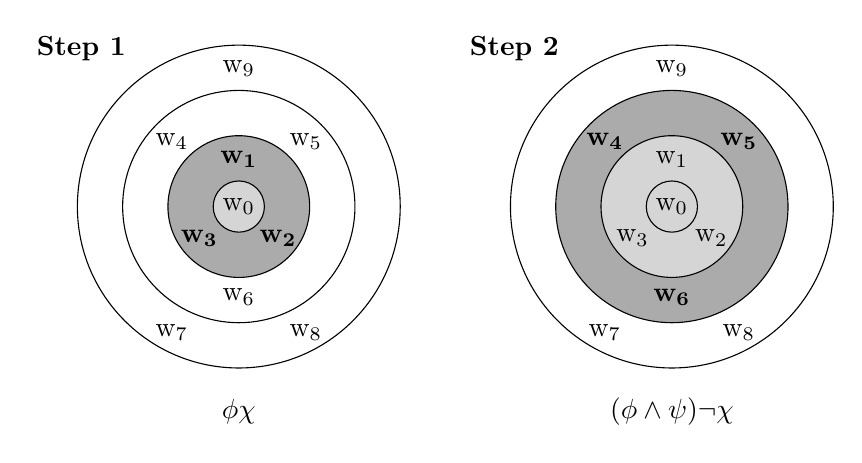
\begin{tikzpicture}
	\coordinate (O) at (0,0);
    \node at (-2,2) {\textbf{Step 1}};
	\draw[fill=white] (O) circle (2.05);
	\draw[fill=white] (O) circle (1.475);
	\draw[fill=gray!66] (O) circle (0.9);
	\draw[fill=gray!33] (O) circle (0.325)node {w\textsubscript{0}};

	\node at (0,0.6) {\textbf{w\textsubscript{1}}};
	\node at (0.5,-0.4) {\textbf{w\textsubscript{2}}};
	\node at (-0.5,-0.4) {\textbf{w\textsubscript{3}}};
	
	\node at (-0.85,0.825) {w\textsubscript{4}};
	\node at (0.85,0.825) {w\textsubscript{5}};
	\node at (0,-1.15) {w\textsubscript{6}};
	
	\node at (-0.85,-1.6) {w\textsubscript{7}};
	\node at (0.85,-1.6) {w\textsubscript{8}};
	\node at (0,1.75) {w\textsubscript{9}};
	
	\node at (0,-2.6) {$\phi\cf\chi$};
	
	
	\begin{scope}[xshift=5.5cm]
		\coordinate (O) at (0,0);
        \node at (-2,2) {\textbf{Step 2}};
    \draw[fill=white] (O) circle (2.05);
	\draw[fill=gray!66] (O) circle (1.475);
	\draw[fill=gray!33] (O) circle (0.9);
	\draw[fill=gray!33] (O) circle (0.325)node {w\textsubscript{0}};

	\node at (0,0.6) {{w\textsubscript{1}}};
	\node at (0.5,-0.4) {{w\textsubscript{2}}};
	\node at (-0.5,-0.4) {{w\textsubscript{3}}};
	
	\node at (-0.85,0.825) {\textbf{w\textsubscript{4}}};
	\node at (0.85,0.825) {\textbf{w\textsubscript{5}}};
	\node at (0,-1.15) {\textbf{w\textsubscript{6}}};
	
	\node at (-0.85,-1.6) {w\textsubscript{7}};
	\node at (0.85,-1.6) {w\textsubscript{8}};
	\node at (0,1.75) {w\textsubscript{9}};
	
	\node at (0,-2.6) {$(\phi\land\psi)\cf\neg\chi$};
	\end{scope}
\end{tikzpicture}
\caption{Quantificational domains for Sobel sequences according to \citepos{Fintel2001} semi-dynamic strict conditional analysis. For all worlds $w_n$: If $n\geqslant1$, then $\phi=1$ is true for $w_n$, and if $n\geqslant 4$, then $\psi=1$ holds true for $w_n$. Non-antecedent worlds present within the modal horizon are shaded in the lighter grey.}\labfig{fintel-SS-repeat}
\end{figure}

\noindent Crucially, the modal horizon does not shrink easily. As such, any world that is incorporated into the modal horizon stays there for future evaluations until the modal horizon is either reset or shrunk (with some considerable effort). In this manner, the modal horizon fulfils the role handled by modal subordination for variably-strict semantics (as previously laid out in \refsec{modal}). For reverse Sobel sequences, this would entail that the $\phi$-conditional quantifies over the $\phi\land\psi$-worlds that were introduced into the modal horizon by the preceding $\phi\land\psi$-conditional. It should be noted, however, that contrary to a variably-strict semantics with modal subordination, the conditional does not quantify merely over the closest $\phi\land\psi$-worlds, but also over any other equally close or closer $\phi$-worlds.\footnote{Note, however, that this makes little difference, since the $\phi\land\psi$-worlds are the critical worlds that cause contradictory readings.} This process was illustrated in \reffig{fintel-rSS}, as repeated below in \reffig{fintel-rSS-repeat}.
\begin{figure}[!htb]
\input{content/graphics/fintel-rSS.tikz}
\caption{Quantificational domains for reverse Sobel sequences according to \citepos{Fintel2001} semi-dynamic strict conditional analysis. For all worlds $w_n$: If $n\geqslant1$, then $\phi=1$ is true for $w_n$, and if $n\geqslant 4$, then $\psi=1$ holds true for $w_n$. Non-antecedent worlds present within the modal horizon are shaded in the lighter grey.}\labfig{fintel-rSS-repeat}
\end{figure}

As such, for a (semi-)dynamic strict semantics, the modal horizon effectively takes the place of aboutness topics and modal subordination to derive the contradictory readings of infelicitous reverse Sobel sequences. It should be noted that neither \textcite{Fintel2001} nor \textcite{Gillies2007} differentiated between causal and acausal (reverse) Sobel sequences. We would posit, however, that this distinction is easily incorporated by simply adopting \textcite{Bennett2003} and \citepos{Arregui2009} view on how causality impacts world similarity orderings. This has only one immediate consequence: We require \citepos{Klecha2014,Klecha2015} imprecision-based semantics for a felicitous analysis of regularly ordered Sobel sequences, as the expansion to include $\phi$-worlds would already include $\phi\land\psi$-worlds since they are of equal world similarity to the evaluation world.

However, with this basic framework, we are left with all reverse Sobel sequences being rendered infelicitous---similar to our status at the end of \refsec{modal}. As such, we must introduce the role contrastive stress plays into this system.

\subsection{The Effect of Contrastively Stressed Auxiliary Verbs}\labsec{strict-aux}
In this section, we do not motivate our treatment of contrastively stressed TAM morphology in the antecedent along the lines of contrastively stressed bound pro-forms. For the appropriate motivation, we refer back to \refsec{proform}. In addition to our assumptions regarding the nature of TAM morphology and its interaction with contrastive stress, we additionally inherit the assumption from \refsec{showitworks} that non-counterfactual conditional semantics do not make use of a differentiated world closeness ordering beyond the separation of indicative worlds from future-less-vivid worlds.

Recall that a contrast in TAM-morphology in the antecedent actually corresponds to a contrast in quantificational domains. It does this by contrasting two identity functions who are restricted in their domain to the appropriate set of antecedent worlds. A contrast is successful iff the two contrasted domains are entirely disjoint. The abstract LFs of a reverse Sobel sequences were given in \refex{identityw} and are repeated below as \refex{identityw-repeat}.
\pex\label{ex:identityw-repeat}
\a If $[\lambda w_s. \phi(\text{\textbf{\color{black}\scshape id\textsubscript{domain-b}}}(w))\land \psi(\text{\color{black}\scshape id\textsubscript{domain-b}}(w))]$, (then) $[\lambda w_s.\neg\chi(w)]$.
\a If $[\lambda w_s. \phi(\text{\textbf{\color{black}\scshape id\textsubscript{domain-a}}}(w))]$, (then) $[\lambda w_s.\chi(w)]$.
\xe
Here, the question is what domain A and domain B should correspond to. In a variably-strict semantics, the answer was quite apparent: They correspond to the set of the closest $\phi$-worlds and the set of the closest $\phi\land\psi$-worlds, respectively, as these were the respective standard domains of quantification if modal subordination were to be dismissed as a factor. For our (semi-)dynamic strict semantics, the answer is a bit more muddled and a few possible candidates come to mind. 

One of the most intuitive ones would be that they correspond to the respective states of the modal horizon. Here, two sub-possibilities come into play: The first option would be to contrast the two states of the modal horizon as they should be according to standard (semi-)dynamic strict semantics. The second option would be to contrast the two minimal states of the modal horizon as they would be if the reverse Sobel sequence's conditionals were found in contextless isolation. However, neither option has any chance at succeeding. Due to the nature of how the modal horizon expands, one state of the modal horizon must always be either subset of or superset to any other state of the modal horizon. As such, they may never be disjoint.

Another intuitive candidate would be that they correspond to the respective states of the modal horizon intersected by all worlds compatible with the concurrent antecedent. Here, the same two sub-possibilities come into play. The first option---that we intersect the antecedent worlds with the standard respective states of the modal horizon---would fail for the same reason as why our first intuitive candidate could not succeed: The $\phi$-conditional's modal horizon state intersected by all $\phi$-worlds would contain the $\phi\land\psi$-worlds introduced by the previous conditional. Therefore, the two contrasting domains could never be disjoint, as one would always be a subset of the other. This can easily be seen by comparing the areas shaded in a dark grey in \reffig{fintel-rSS-repeat}. The second option---that we intersect the antecedent worlds with the states of the modal horizon as if the conditionals were found in contextless isolation---is more promising however. In that case, the two contrasting domains would merely correspond to the closest $\phi$-worlds and the closest $\phi\land\psi$-worlds (i.e.,~the areas shaded in a dark grey in \reffig{fintel-SS-repeat}).

As such, the contrasted domains A and B would correspond to the same domains as in the variably-strict semantics in \refsec{proform} in \refex{identityw-variably-strict}, as repeated below in \refex{identityw-variably-strict-repeat}.
\pex\label{ex:identityw-variably-strict-repeat}
\a If $[\lambda w_s. \phi(\text{\textbf{\color{black}\scshape id\textsubscript{closest-$\phi\land\psi$}}}(w))\land \psi(\text{\color{black}\scshape id\textsubscript{closest-$\phi\land\psi$}}(w))]$, (then) $[\lambda w_s.\neg\chi(w)]$.
\a If $[\lambda w_s. \phi(\text{\textbf{\color{black}\scshape id\textsubscript{closest-$\phi$}}}(w))]$, (then) $[\lambda w_s.\chi(w)]$.
\xe
The formal implementation of which is shown in \refex{strict-contrast-demo}:
\pex\label{ex:strict-contrast-demo}
\a $\intension{If $\phi$ and $\psi$, not $\chi$}=[\lambda w_s.\hspace{1mm}\forall v\in f^{\phi\land\psi}_\sigma(w)\cap [\lambda w'_s.\phi(\text{\textbf{\color{black}\scshape id\textsubscript{closest-$\phi\land\psi$}}}(w'))$\\\emptyfill$\land\psi(\text{\textbf{\color{black}\scshape id\textsubscript{closest-$\phi\land\psi$}}}(w'))]\hspace{0.5mm}[\neg\chi(v)]\hspace{1mm}]]]$
\a $\intension{If $\phi$, $\chi$}=[\lambda w_s.\hspace{1mm}\forall v\in f^{\phi}_\sigma(w)\cap [\lambda w'_s.\phi(\text{\textbf{\color{black}\scshape id\textsubscript{closest-$\phi$}}}(w'))]\hspace{0.5mm}[\neg\chi(v)]\hspace{1mm}]]]$
\xe

This would mean that the contrastive stress, in a (semi-)dynamic strict semantics, can only work if it is to be taken as a command to shrink the modal horizon. Intuitively speaking, one can think of it in the following way: After having spoken about some possibility of $\phi\land\psi$, you wish to discard the notion of $\phi\land\psi$ as a relevant topic of conversation. To do this, you contrast the worlds of $\phi\land\psi$ against the worlds you now wish to speak about: The $\phi$-worlds that are closer to the evaluation world than the closest $\phi\land\psi$-worlds. To establish this contrast, the contrasting domains must be disjoint, which is only possible if the modal horizon were to shrink to exclude any worlds less similar than the closest $\phi$-worlds. This prompts the discourse participants to either accommodate this request---and shrink their modal horizon for the evaluation of the current conditional---or not. The latter would yield a contradiction and is therefore the dispreferred solution, as a more charitable and non-contradictory discourse move has been proposed.

Having shown how our assumptions regarding how contrastive stress on TAM morphology in the antecedent of conditionals interact with the basic principles of a (semi-)dynamic strict semantics, we now explore in the next section (i.e.,~\refsec{strict-retrodiction}) if and how we derive the desired patterns of (in-)felicity for reverse Sobel sequences.

\subsection{Retrodiction: Accounting for All Available Data With a Dynamic Strict Semantics}\labsec{strict-retrodiction}
In order to test whether or not the model posited in \refsec{strict-horizon} and \refsec{strict-aux} makes accurate predictions concerning the (in-)felicity of reverse Sobel sequences and regularly ordered Sobel sequences, we must first recall two important patterns of (in-)felicity: First, that all regularly ordered Sobel sequences are felicitous. Second, that the felicity of reverse Sobel sequences is dependent upon contrastive stress and three subordinate factors: causality, counterfactuality, and denigration. We established and summarised this in \refsec{introspection} in \reftab{ourdata}, repeated below as \reftab{ourdata-repeat2}.
\begin{table}[!htb]
\input{content/tables/mydata}\labtab{ourdata-repeat2}
\end{table}

We would like to note that, due to the similarities between the modes proposed in \refsec{proform} and \refsec{strict-aux}, much of the reasoning here is near duplicate to the reasoning found in \refsec{showitworks}. As such, most of the explanations are kept briefer than the explanations found in \refsec{showitworks}.

In fact, since our explanations for the felicity of regularly ordered Sobel sequences are virtually identical, we see no need to duplicate them here. Instead, we refer to \refsec{showitworks-ss} for details. In essence, we simply keep \citepos{Fintel2001} standard semantics for Sobel sequences but must introduce imprecision and precisification to account for any non-counterfactual or causal Sobel sequences due to the restrictions we set upon non-counterfactual semantics in \refsec{stric-rss-demo}, having inherited the structural restrictions we have placed upon non-counterfactual semantics from \refsec{showitworks} (i.e.,~that indicative and future-less-vivid conditionals each quantify over a domain of worlds that is internally unstructured and not subdivided into further degrees of world closeness).

\subsubsection{Reverse Sobel Sequences}\labsec{stric-rss-demo}
First, let us examine the effect of counterfactuality of $\phi\land\psi$ (again, we loop back to the effect of non-counterfactuality only later on). The example reverse Sobel sequences contrasting counterfactual reverse Sobel sequences with non-counterfactual ones, \refex{matchtomorrow} and \refex{match-repeat4}, are repeated below as \refex{doomsday-z} and \refex{doomsday-zz}, respectively.
\ex\context{Concerning a dry match in a room with a large open source of water.}
    If I struck this match tomorrow and it was wet, it wouldn't light; \#but if I \MakeUppercase{were} to strike this match tomorrow, it would light.\labex{doomsday-z}
\xe
\ex\context{Holding up a dry match, with no water around.}If I had struck this match and it had been soaked, it would not have lit. But if I \MakeUppercase{had} struck this match, it would have lit.\\%
\emptyfill(adapted from \textcite[p.~106]{Stalnaker1968} by \textcite[p.~487]{Lewis2018})\labex{doomsday-zz}
\xe

In order derive a felicitous reverse Sobel sequence, we require two disjoint domains when we intersect the modal horizon with the closest antecedent worlds. In the case of counterfactual conditionals, this is determined by whether or not the closest $\phi\land\psi$-worlds and the closest $\phi$-worlds are of unequal world similarity. Whether or not this is actually the case is dependent upon the factor of causality.

As extensively covered in \refsec{CSS}, assuming a world similarity metric in the spirit of \textcite{Bennett2003} and \textcite{Arregui2009} would postulate that the closest $\phi\land\psi$-worlds and the closest $\phi$-worlds are equal in similarity if $\phi$ precedes $\psi$ on some causal chain of events. As such, if $\phi$ does precede $\psi$ on some causal chain of events, then $f^{\phi\land\psi}_\sigma(w)\cap D_{\text{closest-}\phi\land\psi}\subseteq f^{\phi}_\sigma(w)\cap D_{\text{closest-}\phi}$ necessarily holds true, which would entail $(f^{\phi\land\psi}_\sigma(w)\cap D_{\text{closest-}\phi\land\psi})\cap(f^{\phi}_\sigma(w)\cap D_{\text{closest-}\phi})\neq\emptyset$.\footnote{In fact, as we attempt to evaluate reverse Sobel sequences in a felicitous manner by rendering their domains disjoint via the shrinking of the modal horizon---shifting from $f^{\phi\land\psi}$ to $f^{\phi}$---these inferences also hold true for the general domains $D_\phi$ and $D_{\phi\land\psi}$. Whilst the use of $D_\phi$ and $D_{\phi\land\psi}$ would be truer to the underlying mechanism of the (semi-)dynamic strict semantics, we have opted for the domains being restricted to the closest available antecedent worlds to emphasise the shrinking process. This remains true for all inferences and entailments in this section.} As such, no successful contrast is possible, preventing the shrinking of the modal horizon. That is, even if the modal horizon were to shrink, we would still arrive at a contradictory statement. As such, a causal counterfactual reverse Sobel sequence is necessarily infelicitous. This was exemplified with the causal counterfactual reverse Sobel sequence in \refex{matchsnapcf}, repeated below as \refex{wonderwoman-repeat}.
\ex\context{Holding up a dry match (with no water around).}If I had struck this match and it had snapped, it would not have lit. \#But if I \MakeUppercase{had} struck this match, it would have lit.\labex{wonderwoman-repeat}
\xe

If, on the other hand, $\phi$ does not precede $\psi$ on some causal chain of events, the closest $\phi\land\psi$-worlds would not count amongst the closest $\phi$-worlds, as $\psi$ would introduce an additional level of world dissimilarity. Therefore, for acausal counterfactual reverse Sobel sequences, $f^{\phi\land\psi}_\sigma(w)\cap D_{\text{closest-}\phi\land\psi}\not\subseteq f^{\phi}_\sigma(w)\cap D_{\text{closest-}\phi}$ necessarily holds true, which, in turn, taking into account how world similarity orderings work, would entail that $(f^{\phi\land\psi}_\sigma(w)\cap D_{\text{closest-}\phi\land\psi})\cap(f^{\phi}_\sigma(w)\cap D_{\text{closest-}\phi})=\emptyset$. As such, as the two domains of quantification are necessarily disjoint, the modal horizon may be shrunk, ensuring that contrastively stressed acausal counterfactual reverse Sobel sequences are typically felicitous. This explains why acausal counterfactual reverse Sobel sequence such as \refex{match-repeat4}, repeated below as \refex{greenlantern-repeat} are rendered felicitous.
\ex\context{Holding up a dry match, with no water around.}If I had struck this match and it had been soaked, it would not have lit. But if I \MakeUppercase{had} struck this match, it would have lit.\\%
\emptyfill(adapted from \textcite[p.~106]{Stalnaker1968} by \textcite[p.~487]{Lewis2018})\labex{greenlantern-repeat}
\xe

With this, we turn towards the factor of non-counterfactuality. Similarly to the variably-strict semantics variant of this model, this part makes less of a prediction for indicative reverse Sobel sequences rather than it imposes restrictions on how indicative semantics are to implemented. As \textcite{Fintel2001} did not extend his analysis to non-counterfactuals, any extensions to this effect must be such that all indicative worlds and all future-less-vivid worlds each occupy a single sphere of world similarity, respectively. This is needed to ensure that $(f^{\phi\land\psi}_\sigma(w)\cap D_{\text{closest-}\phi\land\psi})\cap(f^{\phi}_\sigma(w)\cap D_{\text{closest-}\phi})\neq\emptyset$ holds true for any non-counterfactual reverse Sobel sequence, as all (non-denigrated) non-counterfactual reverse Sobel sequences have been shown to be infelicitous, as demonstrated with \refex{matchtomorrow} and \refex{matchsnapnocf}, repeated below as \refex{doomsday1-repeat} and \refex{doomsday2-repeat}, respectively.
\ex\context{Concerning a dry match in a room with a large open source of water.}
    If I struck this match tomorrow and it was wet, it wouldn't light; \#but if I \MakeUppercase{were} to strike this match tomorrow, it would light.\labex{doomsday1-repeat}
\xe
\ex\context{Holding up a dry match (with no water around).}
If I struck this match and it snapped, it would not light. \#But if I \MakeUppercase{were} to strike this match, it would light.\labex{doomsday2-repeat}
\xe 
We refer to \refsec{showitworks} for further details. With this, we may take stock of the data accounted so far. We can accurately predict that non-counterfactual reverse Sobel sequences and causal reverse Sobel sequences are infelicitous, as either factor would ensure that both conditionals' domains could never be disjoint. Acausal counterfactual reverse Sobel sequences are the only conditionals whose domains of quantification are ensured to be disjoint by the very nature of how we rank worlds according to their closeness to some evaluation world. This is summarised in \reftab{less-confused-maribel-table-rssonly-fintel}.
\begin{table}[!htb]
    \caption{Currently accounted for empirical data regarding reverse Sobel sequences, broken down by causality and counterfactuality, omitting denigration as a factor, with example numbers that exemplify each reverse Sobel sequence condition. Contrastive stress on the auxiliary verb is assumed for all reverse Sobel sequences.}
\begin{tabular}{lcccc}\toprule
                &   \multicolumn{2}{c}{Acausal}     &  \multicolumn{2}{c}{Causal}\\
                & \multicolumn{1}{c}{Non-Counterfactual}  &   \multicolumn{1}{c}{Counterfactual}    & \multicolumn{1}{c}{Non-Counterfactual}  &   \multicolumn{1}{c}{Counterfactual}\\\midrule
                rSS   &   \#\refex{matchtomorrow}  & \checkmark\refex{match-repeat4}  &    \#\refex{matchsnapnocf} & \#\refex{matchsnapcf}  \\
                \bottomrule
\end{tabular}\labtab{less-confused-maribel-table-rssonly-fintel}
\end{table}

With this, we move on to the factor of denigration, which serves as a catch-all rescue operation that renders any contrastively stressed reverse Sobel sequence felicitous. Here, we, again, reason along the lines of the respective part of \refsec{showitworks}. We would argue that denigration along the lines of \refex{acausalncfdenigrated}, \refex{causalncfdenigrated}, \refex{match-acausal-denigrated}, and \refex{match-causal-denigrated}, which are repeated below as \refex{superman1-repeat}, \refex{superman2-repeat}, \refex{superman3-repeat}, and \refex{superman4-repeat}, respectively, causes felicity in reverse Sobel sequences by imposing context-/relevance-based restrictions on the reverse Sobel sequences' domains of quantification \parencites[see][]{Fintel1994}{Reimer1998}[amongst many others]{Stanley2000}.
\pex
\a\context{Concerning a dry match in a room with a large open source of water.}
    If I struck this match tomorrow and it was wet, it wouldn't light. But there is little chance of this match becoming wet; so, if I \MakeUppercase{were} to strike this match tomorrow, it would light.\labex{superman1-repeat}
\a\context{Holding up a dry match (with no water around).}If I struck this match and it snapped, it would not light. But the chances of me snapping a match are really, really low; so, if I \MakeUppercase{were} to strike this match, it would light.\labex{superman2-repeat}
\a\context{Holding up a dry match, with no water around}If I had struck this match and it had been soaked, it would not have lit. But, as we know, this match is dry, so if I \MakeUppercase{had} struck this match, it would have lit.\labex{superman3-repeat}
\a\context{Holding up a dry match (with no water around).}If I had struck this match and it had snapped, it wouldn't have lit. But the chances of the match breaking would've been very, very, \MakeUppercase{very} low, since I know what I'm doing. So, if I \MakeUppercase{had} struck this match, it would have lit.\labex{superman4-repeat}
\xe

Effectively, denigrating the possibility of $\psi$ removes all $\psi$-worlds from any conditional not actively evaluating the consequences of $\psi$. As all $\psi$-worlds are removed from the closest $\phi$-worlds (if, in fact, there were any), there cannot be an overlap between the closest $\phi\land\psi$-worlds and the closest $\phi$-worlds. Formally speaking, $(f^{\phi\land\psi}_\sigma(w)\cap D_{\text{closest-}\phi\land\psi})\cap((f^{\phi}_\sigma(w)\cap D_{\text{closest-}\phi})\setminus D_\psi)=\emptyset$ is a tautology, which ensures that any denigrated reverse Sobel sequence is felicitous, as the contrastive stress succeeds and all worlds that might cause a contradictory reading are removed from the proverbial and non-proverbial equation.

With this, we would yield correct predictions for all currently known cases of reverse Sobel sequences, as categorised by \reftab{ourdata-repeat}---be they felicitous or infelicitous reverse Sobel sequences. This is summarised below in \reftab{ourdata-rssonly-fintel}.
\begin{table}[!htb]
\caption{Current accounted for empirical data regarding reverse Sobel sequences, broken down by causality, counterfactuality, and either implicit or explicit denigration, with example numbers that exemplify each reverse Sobel sequence condition. Contrastive stress on the auxiliary verb is assumed for all reverse Sobel sequences.}
\resizebox{\textwidth}{!}{
    \begin{tabular}{lcccccccc}\toprule
                &   \multicolumn{4}{c}{Acausal}     &  \multicolumn{4}{c}{Causal}\\
                & \multicolumn{2}{c}{Non-Counterfactual}  &   \multicolumn{2}{c}{Counterfactual}    & \multicolumn{2}{c}{Non-Counterfactual}  &   \multicolumn{2}{c}{Counterfactual}\\
                & Non-Denigrated & Denigrated  & Non-Denigrated & Denigrated   & Non-Denigrated & Denigrated & Non-Denigrated & Denigrated\\\midrule
          rSS   &   \#\refex{matchtomorrow}  & \checkmark\refex{acausalncfdenigrated}  & \checkmark\refex{match-repeat4}  &   \checkmark\refex{match-acausal-denigrated}  &   \#\refex{matchsnapnocf} & \checkmark\refex{causalncfdenigrated} &   \#\refex{matchsnapcf}    &   \checkmark\refex{match-causal-denigrated}\\
          \bottomrule
    \end{tabular}}\labtab{ourdata-rssonly-fintel}
\end{table}

\noindent Furthermore, given that the account for the felicity of regularly ordered Sobel sequences in this (semi-)dynamic strict framework does not meaningfully differ from the account provided for the variably-strict framework in \refsec{showitworks-ss}, as previously mentioned, we would also correctly derive the universal felicity of regularly ordered Sobel sequences. This is summarised in \reftab{ourdata-anotherrepeat-fintel}.
\begin{table}[!htb]
\input{content/tables/mydata-ssrss}\labtab{ourdata-anotherrepeat-fintel}
\end{table}\vspace{-10mm}

\section{Intermediate Conclusion}
With this, we can account for the entire (in-)felicity distribution concerning reverse Sobel sequences with either a variably-strict semantics (as shown in \refsec{showitworks}) or a (semi-)dynamic strict semantics (as shown in \refsec{strict-retrodiction}). Naturally, this poses an interesting issue: As the variably-strict semantics and and the (semi-)dynamic strict semantics are equally capable of accounting for the infelicity and felicity of the appropriate reverse Sobel sequences, there is no inherent advantage of one account over the other. As such, it would appear Sobel sequences and reverse Sobel sequences turn into a non-issue for the debate between the two fundamental approaches to modelling conditional semantics. As such, the debate must focus on other deciding phenomena in the future to reach a final verdict.
